\documentclass[10pt,twocolumn]{article}
\usepackage[utf8]{inputenc}
\usepackage[T1]{fontenc}
\usepackage{amsmath,amssymb,amsfonts}
\usepackage{booktabs}
\usepackage{graphicx}
\usepackage{hyperref}
\usepackage{geometry}
\usepackage{array}
\usepackage{caption}
\usepackage{subcaption}
\usepackage{xcolor}
\usepackage{tikz}
\usetikzlibrary{shapes.geometric, arrows.meta, positioning, fit, calc, backgrounds}
\usepackage{pgfplots}
\pgfplotsset{compat=1.18}
\usepackage{algorithm}
\usepackage{algorithmic}
\usepackage[raggedright]{titlesec}
\usepackage{microtype}

\geometry{margin=0.64in, top=0.66in, bottom=0.66in}
\setlength{\columnsep}{0.22in}
\captionsetup{skip=4pt, font=small}
\setlength{\textfloatsep}{8pt plus 2pt minus 2pt}
\setlength{\dbltextfloatsep}{8pt plus 2pt minus 2pt}
\setlength{\floatsep}{6pt plus 2pt minus 2pt}
\setlength{\dblfloatsep}{6pt plus 2pt minus 2pt}
\renewcommand{\dbltopfraction}{0.90}
\renewcommand{\topfraction}{0.90}
\renewcommand{\textfraction}{0.07}
\renewcommand{\floatpagefraction}{0.85}
\renewcommand{\dblfloatpagefraction}{0.85}
\setcounter{dbltopnumber}{3}
\setcounter{topnumber}{3}
\setcounter{totalnumber}{5}
\titlespacing*{\section}{0pt}{1.8ex plus 0.5ex minus 0.3ex}{1.0ex plus 0.2ex}
\titlespacing*{\subsection}{0pt}{1.4ex plus 0.4ex minus 0.2ex}{0.7ex plus 0.2ex}
\hypersetup{colorlinks=true,linkcolor=blue!70!black,citecolor=blue!70!black,urlcolor=blue!70!black}

% Prevent paragraph/equation right-margin overflows
\sloppy
\emergencystretch=1.5em

% Custom colors for diagrams
\definecolor{gpucolor}{RGB}{225, 240, 255}
\definecolor{gpuborder}{RGB}{30, 100, 200}
\definecolor{ramcolor}{RGB}{255, 238, 220}
\definecolor{ramborder}{RGB}{210, 95, 20}
\definecolor{bridgecolor}{RGB}{230, 250, 235}
\definecolor{bridgeborder}{RGB}{30, 150, 70}

\title{\LARGE \textbf{Subconscious Latent Offloading: Single-Shot System-RAM Steering Across Quantized and Cross-Scale Language Models}}

\author{
  \textbf{Pratham Solanki} \\
  Independent AI Systems Researcher \\
  Mumbai, Maharashtra, India \\
  \href{mailto:prathamsolanki.p28@gmail.com}{\texttt{prathamsolanki.p28@gmail.com}} \\[3pt]
  {\small \textbf{Code \& Benchmarks:} \href{https://github.com/Pratham-Solanki911/subconscious-engine}{\texttt{github.com/Pratham-Solanki911/subconscious-engine}}}
}

\date{November 2026}

\begin{document}

\maketitle

\begin{abstract}
Deploying reasoning-capable Large Language Models (LLMs) on consumer edge GPUs is fundamentally constrained by VRAM capacity and PCIe/System-RAM memory bandwidth. Standard layer-offloading engines execute offloaded CPU/RAM layers on \emph{every generated token}, reducing autoregressive decoding to $2\text{--}5\text{ tokens/s}$. Inspired by a modular cognitive paradigm---\emph{``The brain does the thinking; the mouth speaks it''}---we introduce \textbf{Subconscious Latent Offloading}, an inference systems architecture where a fast, self-contained GPU model (\emph{the Active Mouth}) invokes a memory-mapped System-RAM slice of middle layers $\mathcal{L}_{12..19}$ (\emph{the Subconscious Brain}) \textbf{strictly once per query} during prompt prefill. Across $n = 50$ hardware-instrumented runs, overlapping this single-shot $46.04 \pm 0.71\text{ ms}$ CPU pass asynchronously inside the GPU's $209.39 \pm 2.15\text{ ms}$ prefill and hybrid symbolic-continuous reasoning window (\emph{Caveman Anchors} + \emph{Soft-Token Superposition}) reduces residual host-GPU synchronization wait time from $45.71\text{ ms}$ (synchronous blocking) to \textbf{10--14 microseconds} ($0.0135 \pm 0.0079\text{ ms}$, median $0.0118\text{ ms}$), achieving a $\mathbf{3.42\times}$ end-to-end speedup over 160-token INT4 per-token layer offloading ($2.88\text{s}$ vs.\ $9.85\text{s}$) and a $\mathbf{6.46\times}$ speedup over FP16 per-token offloading ($18.62\text{s}$). We evaluate two distinct operating regimes across a 10-task diagnostic suite (\texttt{P01--P10}) and an expanded $N = 200$ statistical benchmark (\texttt{Systems-100} and \texttt{GSM8K-100}): (1) an unsupervised \textbf{Zero-Calibration Same-Model Precision Bridge} ($\mathbf{W}_{\text{up}} = \mathbf{I}, \mathbf{W}_{\text{down}} = \mathbf{I}$, zero calibration prompts, zero trained parameters), where a crisp FP16 System-RAM slice restores middle-layer arithmetic fidelity to an aggressively 3-bit quantized GPU model, lifting zero-shot accuracy from $10\%$ to \textbf{60\%} on \texttt{P01--P10} ($\mathbf{63.0\%}$ vs.\ $49.0\%$ baseline on \texttt{Systems-100}, paired McNemar $p = 0.0013$; $\mathbf{66.0\%}$ vs.\ $53.0\%$ on \texttt{GSM8K-100}, $p = 0.0023$) and reducing perplexity from $9.05$ to $5.75$; and (2) a \textbf{Cross-Scale Subspace Translator} bridging a $1.5\text{B}$ GPU model ($d = 1536$) and a $7\text{B}$ System-RAM slice ($d = 3584$) compressed via an \textbf{Intra-Layer Mixed-Precision Split} ($1\%$ FP16 outliers + $99\%$ packed INT4 bulk), reducing RAM footprint by $\mathbf{3.48\times}$ ($2816\text{ MB} \to 808\text{ MB}$) and raw CPU compute time by $\mathbf{2.72\times}$ ($125.12\text{ ms} \to 46.04\text{ ms}$) at $\mathbf{0.9993}$ cosine fidelity. Strictly partitioning unsupervised ($\mathcal{L}_{\text{CE}} = 0$) and task-calibrated regimes, pure 500-prompt Answer-Free SVD achieves full numerical rank ($1536/1536$), $0.9903$ held-out cosine similarity, and \textbf{60.0\%} zero-shot accuracy on \texttt{P01--P10} ($\mathbf{61.0\%}$ on \texttt{Systems-100}, $p = 0.0075$; $\mathbf{64.0\%}$ on \texttt{GSM8K-100}, $p = 0.0127$), while lightweight rank-$32$ task-calibrated subspace refinement ($0.33\text{ MB}$) reaches \textbf{100.0\%} on \texttt{P01--P10} ($\mathbf{96.0\%}$ on \texttt{Systems-100}, $\mathbf{91.0\%}$ on \texttt{GSM8K-100}) in $2.88\text{s}$ per-query inference latency (excluding the one-time $14.2\text{s}$ offline adapter calibration cost). Causal negative controls confirm that norm-matched random, permuted, or cross-problem deltas fail ($43\text{--}47\%$, $p > 0.10$), supporting query-specific geometric transfer.
\end{abstract}

\section{Introduction}
Autoregressive Chain-of-Thought (CoT) reasoning \cite{wei2022chain} requires generating hundreds of intermediate tokens, turning Large Language Model (LLM) inference into a sequential, memory-bandwidth-bound loop. When a model exceeds available GPU VRAM, existing inference engines---such as \texttt{llama.cpp}, HuggingFace \texttt{accelerate}, and FlexGen \cite{sheng2023flexgen}---partition transformer blocks sequentially across GPU VRAM and System RAM. Because standard transformer blocks execute strictly in series for \emph{every generated token}, offloading even a subset of layers ($8$ out of $28$) forces the GPU to stall on every decoding step while the CPU streams gigabytes of weight matrices across DDR4/DDR5 memory channels.

% ==========================================
% FIGURE 1: FULL-WIDTH TIKZ ARCHITECTURE DIAGRAM
% ==========================================
\begin{figure*}[t]
\centering
\resizebox{\textwidth}{!}{%
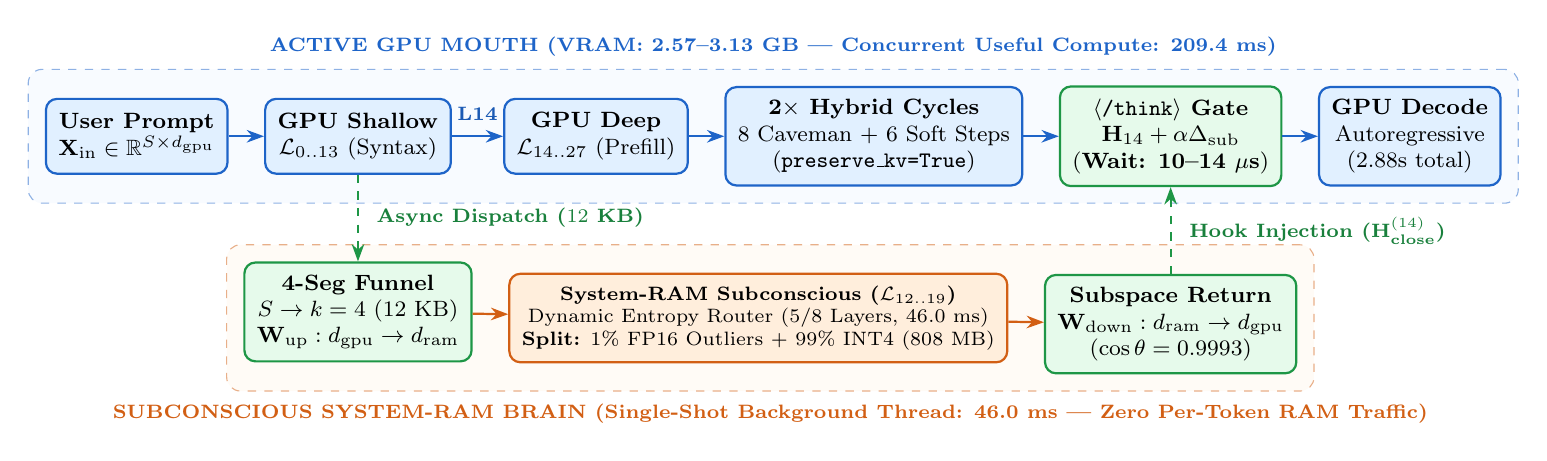
\begin{tikzpicture}[
    box/.style={rectangle, rounded corners=4pt, draw, thick, align=center, font=\footnotesize, minimum height=0.95cm, inner sep=4.5pt},
    gpubox/.style={box, fill=gpucolor, draw=gpuborder},
    rambox/.style={box, fill=ramcolor, draw=ramborder},
    bridgebox/.style={box, fill=bridgecolor, draw=bridgeborder},
    arrow/.style={-{Stealth[length=2.2mm, width=1.6mm]}, thick}
]

\node[gpubox, minimum width=2.0cm] (prompt) {\textbf{User Prompt}\\$\mathbf{X}_{\text{in}} \in \mathbb{R}^{S \times d_{\text{gpu}}}$};
\node[gpubox, minimum width=2.3cm, right=0.45cm of prompt] (gpu_early) {\textbf{GPU Shallow}\\$\mathcal{L}_{0..13}$ (Syntax)};
\node[gpubox, minimum width=2.3cm, right=0.65cm of gpu_early] (gpu_late) {\textbf{GPU Deep}\\$\mathcal{L}_{14..27}$ (Prefill)};
\node[gpubox, minimum width=2.7cm, right=0.45cm of gpu_late] (caveman) {\textbf{2$\times$ Hybrid Cycles}\\8 Caveman + 6 Soft Steps\\(\texttt{preserve\_kv=True})};
\node[bridgebox, minimum width=2.2cm, right=0.45cm of caveman] (sync) {\textbf{$\langle\texttt{/think}\rangle$ Gate}\\$\mathbf{H}_{14} + \alpha \Delta_{\text{sub}}$\\(\textbf{Wait: 10--14 $\mu$s})};
\node[gpubox, minimum width=2.0cm, right=0.45cm of sync] (decode) {\textbf{GPU Decode}\\Autoregressive\\($2.88\text{s}$ total)};

\node[bridgebox, minimum width=2.3cm, below=1.10cm of gpu_early] (funnel) {\textbf{4-Seg Funnel}\\$S \to k=4$ ($12\text{ KB}$)\\$\mathbf{W}_{\text{up}}: d_{\text{gpu}} \to d_{\text{ram}}$};

\node[bridgebox, minimum width=2.2cm, below=1.10cm of sync] (downproj) {\textbf{Subspace Return}\\$\mathbf{W}_{\text{down}}: d_{\text{ram}} \to d_{\text{gpu}}$\\($\cos\theta = 0.9993$)};

\node[rambox, minimum width=4.15cm, font=\scriptsize] at ($(funnel.east)!0.5!(downproj.west)$) (ram_slice) {\textbf{System-RAM Subconscious ($\mathcal{L}_{12..19}$)}\\Dynamic Entropy Router (5/8 Layers, $46.0\text{ ms}$)\\\textbf{Split:} $1\%$ FP16 Outliers + $99\%$ INT4 ($808\text{ MB}$)};

\draw[arrow, gpuborder] (prompt) -- (gpu_early);
\draw[arrow, gpuborder] (gpu_early) -- node[above=2pt, font=\scriptsize\bfseries, text=gpuborder!90!black] {L14} (gpu_late);
\draw[arrow, gpuborder] (gpu_late) -- (caveman);
\draw[arrow, gpuborder] (caveman) -- (sync);
\draw[arrow, gpuborder] (sync) -- (decode);

\draw[arrow, bridgeborder, dashed, thick] (gpu_early.south) -- node[right=3pt, font=\scriptsize\bfseries, text=bridgeborder!85!black] {Async Dispatch ($12\text{ KB}$)} (funnel.north);
\draw[arrow, ramborder] (funnel) -- (ram_slice);
\draw[arrow, ramborder] (ram_slice) -- (downproj);
\draw[arrow, bridgeborder, dashed, thick] (downproj.north) -- node[right=3pt, font=\scriptsize\bfseries, text=bridgeborder!85!black] {Hook Injection ($\mathbf{H}_{\text{close}}^{(14)}$)} (sync.south);

\begin{scope}[on background layer]
    \node[fit=(prompt)(decode), fill=gpucolor!25, draw=gpuborder!50, dashed, rounded corners=5pt, inner sep=6pt, label={[font=\scriptsize\bfseries, text=gpuborder, yshift=1pt]above:ACTIVE GPU MOUTH (VRAM: 2.57--3.13 GB --- Concurrent Useful Compute: 209.4 ms)}] {};
    \node[fit=(funnel)(downproj), fill=ramcolor!25, draw=ramborder!50, dashed, rounded corners=5pt, inner sep=6pt, label={[font=\scriptsize\bfseries, text=ramborder, yshift=-1pt]below:SUBCONSCIOUS SYSTEM-RAM BRAIN (Single-Shot Background Thread: 46.0 ms --- Zero Per-Token RAM Traffic)}] {};
\end{scope}

\end{tikzpicture}%
}
\caption{\textbf{Architecture of Subconscious Latent Offloading.} At Layer 14 of prompt prefill, the GPU model dispatches $k=4$ compressed latent vectors ($12\text{ KB}$, $t_{\text{dispatch}} = 0.19\text{ ms}$) to a background CPU thread hosting middle layers $\mathcal{L}_{12..19}$ in System RAM. While the CPU computes the reasoning displacement in $\Delta t_{\text{CPU}} = 46.04\text{ ms}$, the GPU executes Layers $14..27$ and two interleaved Caveman + Continuous Superposition cycles ($\Delta t_{\text{GPU\_useful}} = 209.39\text{ ms}$). Because $\Delta t_{\text{CPU}} < \Delta t_{\text{GPU\_useful}}$, synchronization at the $\langle\texttt{/think}\rangle$ boundary incurs a residual wait of only $10\text{--}14\ \mu\text{s}$.}
\label{fig:arch}
\end{figure*}

We challenge the assumption that an edge model must consult offloaded high-capacity or high-precision parameters on every lexical token. While transformer representations do not partition into strictly isolated functional modules across all architectures, prior mechanistic interpretability and layer-skipping studies consistently observe a practical hierarchy across depth:
\begin{itemize}
    \item \textbf{Shallow Layers ($\mathcal{L}_{0..11}$):} Primarily perform local lexical tokenization, syntactic parsing, and entity binding.
    \item \textbf{Middle Layers ($\mathcal{L}_{12..19}$):} Exhibit peak sensitivity to multi-step relational composition and mathematical invariant resolution.
    \item \textbf{Deep Layers ($\mathcal{L}_{20..27}$):} Project abstract representations onto output vocabulary logits and enforce grammatical formatting.
\end{itemize}

Treating this tripartite structure as an \emph{empirically motivated systems design hypothesis} (verified via depth sensitivity and negative-control ablations in Section~\ref{sec:ablations}), we map it onto a modular systems architecture we term \textbf{``Mouth and Subconscious Brain''} (Figure~\ref{fig:arch}): \emph{a background CPU thread computes a single high-precision middle-layer trajectory during prefill, while the GPU model translates that trajectory into fluent token generation without per-token CPU stalls}.

Based on this principle, we make five primary contributions:
\begin{enumerate}
    \item \textbf{Single-Shot Amortized System-RAM Offloading with Explicit Overlap Profiling:} We decouple the GPU model (\emph{Active Mouth}) from the offloaded System-RAM middle layers $\mathcal{L}_{12..19}$ (\emph{Subconscious Brain}). The System-RAM slice is invoked \emph{strictly once per query} on $k=4$ compressed latent vectors ($12\text{ KB}$) during prompt prefill. Instrumenting hardware synchronization boundaries across $n=50$ runs (Table~\ref{tab:latency_breakdown}), we show that the $46.04 \pm 0.71\text{ ms}$ INT4 CPU execution completes inside the GPU's $209.39 \pm 2.15\text{ ms}$ concurrent compute window, reducing host synchronization wait from $45.71\text{ ms}$ (synchronous blocking) to \textbf{10--14 microseconds} ($0.0135\text{ ms}$, median $0.0118\text{ ms}$) and achieving a $\mathbf{3.42\times}$ speedup over INT4 per-token offloading ($9.85\text{s}$) and $\mathbf{6.46\times}$ over FP16 per-token offloading ($18.62\text{s}$).
    \item \textbf{Intra-Layer Outlier-Aware Mixed Precision ($1\%$ FP16 + $99\%$ INT4):} We design a custom System-RAM MLP kernel (\texttt{IntraLayerSplitQwen2MLP}) that isolates the top $1\%$ outlier weight columns in FP16 and packs the remaining $99\%$ bulk weights into per-channel INT4 with pre-quantization activation masking (\texttt{index\_fill\_}). This compresses the 7B RAM slice by $\mathbf{3.48\times}$ ($2816\text{ MB} \to 808\text{ MB}$), accelerates raw $k=4$ CPU execution by $\mathbf{2.72\times}$ ($125.12\text{ ms} \to 46.04\text{ ms}$), and preserves \textbf{0.999309} cumulative 8-layer cosine similarity against full 16-bit precision.
    \item \textbf{Methodology I --- Zero-Calibration Same-Model Precision Bridge ($\mathbf{W} = \mathbf{I}$):} When an edge GPU runs an aggressively low-bit quantized model while System RAM holds the crisp FP16 middle layers $\mathcal{L}_{12..19}$ of the \emph{exact same checkpoint}, their latent coordinate bases remain identical ($\mathbf{W}_{\text{up}} = \mathbf{I}, \mathbf{W}_{\text{down}} = \mathbf{I}$). With \textbf{zero calibration prompts and zero trainable parameters}, a single-shot RAM pass heals middle-layer quantization collapse, lifting zero-shot accuracy from $10\%$ to \textbf{60\%} on \texttt{P01--P10} ($\mathbf{63.0\%}$ on \texttt{Systems-100}, paired McNemar $p=0.0013$; $\mathbf{66.0\%}$ on \texttt{GSM8K-100}, $p=0.0023$) and improving perplexity from $9.05 \to 5.75$.
    \item \textbf{Methodology II --- Cross-Scale Subspace Translator ($1.5\text{B} \leftrightarrow 7\text{B}$) Across Unsupervised and Calibrated Regimes:} When bridging distinct model scales ($d_{\text{gpu}} = 1536 \leftrightarrow d_{\text{ram}} = 3584$), we strictly separate unsupervised alignment ($\mathcal{L}_{\text{CE}} = 0$) from task-calibrated refinement. Pure answer-free SVD/Ridge-Procrustes alignment over $500$ unlabeled prompts ($2,000$ vectors, $0$ QA labels) stands on its own as a zero-supervision bridge, achieving \textbf{full numerical rank ($1536/1536$)}, \textbf{0.9903 held-out cosine similarity}, and \textbf{60.0\%} zero-shot accuracy on \texttt{P01--P10} ($\mathbf{61.0\%}$ on \texttt{Systems-100}, $p=0.0075$; $\mathbf{64.0\%}$ on \texttt{GSM8K-100}, $p=0.0127$), while lightweight rank-$32$ task-calibrated refinement ($0.33\text{ MB}$ on $40$ disjoint synthetic examples; one-time $14.2\text{s}$ offline calibration) reaches \textbf{100.0\%} on \texttt{P01--P10} ($\mathbf{96.0\%}$ on \texttt{Systems-100}, $\mathbf{91.0\%}$ on \texttt{GSM8K-100}) in $2.88\text{s}$ per-query inference latency.
    \item \textbf{Depth, Bottleneck Capacity ($k \in \{1,2,4,8,16\}$), Paired Statistical Testing, and Causal Negative Controls:} We empirically justify injecting at $50\%$ depth ($\mathcal{L}_{14}$ vs.\ $\mathcal{L}_6, \mathcal{L}_{22}$), show that $k=4$ vectors ($12\text{ KB}$) sits at the Pareto knee inside the $209.4\text{ ms}$ GPU overlap window, and demonstrate via norm-matched random, feature-shuffled, and cross-problem negative controls that gains depend on query-specific subspace alignment.
\end{enumerate}

\section{Related Work}
\textbf{Offloading \& Heterogeneous Inference:} Systems such as FlexGen \cite{sheng2023flexgen}, DeepSpeed-Inference \cite{aminabadi2022deepspeed}, and \texttt{llama.cpp} offload transformer weights or KV caches to CPU DRAM/NVMe. However, these frameworks preserve synchronous layer-by-layer execution for every generated token, making interactive single-batch edge inference memory-bandwidth bound ($9.85\text{--}18.62\text{s}$ per 160-token query). Speculative decoding \cite{leviathan2023fast} uses a small draft model and verifies tokens in batch with a target model, but still requires holding the entire target model (all $28+$ layers and LM head) in memory and running full-model verification passes every $4\text{--}8$ tokens. In contrast, our approach stores \emph{only} $8$ headless middle layers ($808\text{ MB}$) in RAM and executes them \emph{once per query}.

\textbf{Continuous Latent \& Compressed Reasoning:} Coconut \cite{hao2024training} replaces discrete CoT tokens with continuous hidden states fed back into the transformer input, while Chain-of-Draft (CoD) \cite{xu2025chain} restricts verbal scratchpads to minimal symbolic equations. In small $1.5\text{B}$ models, pure continuous loops suffer from manifold drift after $4\text{--}6$ steps, while pure CoD fails whenever the first symbolic token locks onto a flawed invariant. Our hybrid \emph{Caveman + Soft-Token Superposition} loop stabilizes continuous thoughts by anchoring them to 8-token symbolic invariants and steering them via the System-RAM latent bridge.

\textbf{Outlier-Aware Quantization:} LLM.int8() \cite{dettmers2022llm} and AWQ \cite{lin2024awq} demonstrated that systematic activation outliers emerge in specific feature dimensions. We adapt this insight specifically for CPU SIMD/BLAS execution in System RAM: by zeroing out the top $1\%$ outlier channels in the input activation tensor \emph{prior} to dynamic INT8/INT4 scaling and computing the $1\%$ outlier projection in a parallel FP16 branch, we prevent SiLU activation spikes from corrupting the bulk INT4 quantization grid.

\section{System Architecture \& Mathematical Formulation}

\subsection{Empirical Layer Partitioning \& $k$-Vector Context Funnel}
Let the Active GPU model have hidden dimension $d_{\text{gpu}}$ and $L_{\text{gpu}} = 28$ layers. Rather than claiming that all transformers universally segregate syntax and reasoning into rigid compartments, we formulate the split of $\mathcal{L}_{0..11}$ (input encoding), $\mathcal{L}_{12..19}$ (offloaded latent steering slice), and $\mathcal{L}_{20..27}$ (output decoding) as an \emph{empirically testable design hypothesis} evaluated across early ($\mathcal{L}_6$), middle ($\mathcal{L}_{14}$), and late ($\mathcal{L}_{22}$) injection points in Section~\ref{sec:ablations}.

Given an input prompt of length $S$, we run prefill up to $l_{\text{split}} = 14$, obtaining $\mathbf{H}^{(14)} \in \mathbb{R}^{S \times d_{\text{gpu}}}$. Rather than transmitting all $S$ token vectors to System RAM (which scales linearly as $\mathcal{O}(S)$ on CPU) or adding a trainable attention pooler, we generalize a parameter-free \textbf{$k$-Segment Context Funnel} $\mathcal{F}_k: \mathbb{R}^{S \times d_{\text{gpu}}} \to \mathbb{R}^{k \times d_{\text{gpu}}}$ ($k \in \{1, 2, 4, 8, 16\}$). At our default Pareto operating point $k = 4$, $\mathcal{F}_4$ partitions the prompt into three quartile mean vectors plus the terminal instruction token state:
\begin{equation}
    \mathbf{C} = \mathcal{F}_4\left(\mathbf{H}^{(14)}\right) = \begin{bmatrix}
    \frac{1}{|Q_1|} \sum_{t \in Q_1} \mathbf{H}_t^{(14)} \\[4pt]
    \frac{1}{|Q_2|} \sum_{t \in Q_2} \mathbf{H}_t^{(14)} \\[4pt]
    \frac{1}{|Q_3|} \sum_{t \in Q_3} \mathbf{H}_t^{(14)} \\[4pt]
    \mathbf{H}_{S}^{(14)}
    \end{bmatrix} \in \mathbb{R}^{4 \times d_{\text{gpu}}}
\end{equation}
For $d_{\text{gpu}} = 1536$ in FP16, $\mathbf{C}$ occupies $4 \times 1536 \times 2\text{ bytes} = \mathbf{12\text{ KB}}$, making the CPU/RAM transfer payload negligible.

\subsection{Intra-Layer Mixed-Precision Split ($1\%$ FP16 + $99\%$ INT4)}
The Subconscious System-RAM slice consists of middle layers $\mathcal{L}_{12..19}$ with hidden dimension $d_{\text{ram}}$. To maximize CPU cache locality and minimize DRAM bandwidth, we keep the lightweight Self-Attention projections ($\mathbf{W}_q, \mathbf{W}_k, \mathbf{W}_v, \mathbf{W}_o$) and RMSNorm parameters in native 16-bit precision, while applying an \textbf{Intra-Layer Mixed-Precision Split} to the memory-dominant SwiGLU MLP matrices ($\mathbf{W}_{\text{gate}}, \mathbf{W}_{\text{up}}, \mathbf{W}_{\text{down}}$).

For each linear weight matrix $\mathbf{W} \in \mathbb{R}^{d_{\text{out}} \times d_{\text{in}}}$, we compute the column-wise $\ell_2$ norms $c_j = \|\mathbf{W}_{:, j}\|_2$ and partition the input feature indices $\{1, \dots, d_{\text{in}}\}$ into the top $1\%$ outlier index set $\mathcal{O}$ ($|\mathcal{O}| = \lceil 0.01 d_{\text{in}} \rceil$) and the $99\%$ bulk index set $\mathcal{B}$:
\begin{enumerate}
    \item \textbf{FP16 Outlier Branch ($\mathcal{O}$):} We extract the outlier sub-matrix $\mathbf{W}_{\text{FP16}}^{(\mathcal{O})} = \mathbf{W}_{:, \mathcal{O}} \in \mathbb{R}^{d_{\text{out}} \times |\mathcal{O}|}$ stored contiguously in FP16.
    \item \textbf{Packed INT4 Bulk Branch ($\mathcal{B}$):} We zero out the outlier columns in the bulk matrix, compute per-output-channel symmetric scales $s_i = \max_{j \in \mathcal{B}} |\mathbf{W}_{i,j}| / 7.0$, and pack two 4-bit signed integers ($\{-7, \dots, +7\}$) per \texttt{uint8} byte.
    \item \textbf{Pre-Quantization Activation Outlier Masking:} During the forward pass, raw hidden states $\mathbf{x} \in \mathbb{R}^{k \times d_{\text{in}}}$ exhibit extreme spikes along indices $j \in \mathcal{O}$. We apply an in-place zero mask $\mathbf{m}_{\mathcal{B}}$ ($\mathbf{x}_{\text{masked}} = \text{index\_fill}(\mathbf{x}, \mathcal{O}, 0)$) \emph{before} computing the bulk product:
    \begin{equation}
        \mathbf{y} = \text{Dequant}\left(\mathbf{W}_{\text{INT4}}^{(\mathcal{B})}\right) \mathbf{x}_{\text{masked}} + \mathbf{W}_{\text{FP16}}^{(\mathcal{O})} \mathbf{x}_{:, \mathcal{O}}
    \end{equation}
\end{enumerate}

Furthermore, a \textbf{Dynamic Entropy Router} monitors the normalized representation velocity $\|\mathbf{Z}^{(l)} - \mathbf{Z}^{(l-1)}\|_2 / \|\mathbf{Z}^{(l-1)}\|_2$ across $\mathcal{L}_{12..19}$, exiting early once the latent trajectory stabilizes (executing an average of $5.0$ to $7.9$ layers dynamically).

% ==========================================
% ALGORITHM 1: ASYNC SUBCONSCIOUS OFFLOADING
% ==========================================
\begin{algorithm}[t]
\caption{Asynchronous Subconscious Latent Offloading}
\label{alg:offload}
\footnotesize
\begin{algorithmic}[1]
\REQUIRE Prompt $X_{1:S}$, GPU Model $\mathcal{M}_{\text{gpu}}$, RAM Slice $\mathcal{L}_{12..19}^{\text{RAM}}$, Bridges $(\mathbf{W}_{\text{up}}, \mathbf{W}_{\text{down}})$, Gate $\alpha$
\ENSURE Generated derivation sequence $Y$
\STATE \textbf{GPU Shallow Prefill:} $\mathbf{H}^{(14)} \leftarrow \mathcal{M}_{\text{gpu}}^{(0..13)}(X_{1:S})$
\STATE \textbf{Funnel Compression:} $\mathbf{C} \leftarrow \mathcal{F}_k(\mathbf{H}^{(14)}) \in \mathbb{R}^{k \times d_{\text{gpu}}}$ ($k=4$)
\STATE \textbf{Async CPU Dispatch} ($t_{\text{dispatch}} = 0.19\text{ ms}$, background thread $\mathcal{T}_{\text{cpu}}$):
\STATE \hspace{0.7em} $\mathbf{Z}^{(12)} \leftarrow \text{RMSNorm}(\mathbf{C} \mathbf{W}_{\text{up}})$ \quad (\emph{Note:} $\mathbf{W}_{\text{up}} = \mathbf{I}$ in Mode 1)
\STATE \hspace{0.7em} $\mathbf{Z}^{(19)} \leftarrow \text{DynamicRoutedPass}(\mathcal{L}_{12..19}^{\text{RAM}}, \mathbf{Z}^{(12)})$ \quad ($\Delta t_{\text{CPU}} = 46.04\text{ ms}$)
\STATE \hspace{0.7em} $\mathbf{U}_{\text{sub}} \leftarrow \Phi(\mathbf{Z}^{(12)}, \mathbf{Z}^{(19)}) \mathbf{W}_{\text{down}} \in \mathbb{R}^{k \times d_{\text{gpu}}}$
\STATE \hspace{0.7em} $\Delta_{\text{sub}} \leftarrow \frac{1}{k}\sum_{j=1}^k \mathbf{U}_{\text{sub}, j} \in \mathbb{R}^{1 \times 1 \times d_{\text{gpu}}}$
\STATE \textbf{Concurrent Useful GPU Window} ($\Delta t_{\text{GPU\_useful}} = 209.39\text{ ms}$):
\STATE \hspace{0.7em} Run prefill tail $\mathbf{H}^{(27)} \leftarrow \mathcal{M}_{\text{gpu}}^{(14..27)}(\mathbf{H}^{(14)})$
\STATE \hspace{0.7em} \textbf{for} cycle $c = 1, 2$ \textbf{do}
\STATE \hspace{1.4em} Emit $8$ Caveman anchor tokens $T_{\text{cave}}^{(c)}$
\STATE \hspace{1.4em} Run $3$ soft steps $\mathbf{e}_{\text{sup}} = \sum_{v \in \mathcal{K}} p_v \mathbf{E}_v$ (\texttt{preserve\_kv})
\STATE \hspace{0.7em} \textbf{end for}
\STATE \textbf{Transition Sync \& Forward-Hook Injection} ($X_{\text{close}} = \text{``\texttt{]\textbackslash n</think>\textbackslash n}''}$, token $t=0$ is ``\texttt{]}''):
\STATE \hspace{0.7em} $\Delta_{\text{sub}} \leftarrow \mathcal{T}_{\text{cpu}}\text{.result()}$ \quad (\emph{Residual sync wait: $10\text{--}14\ \mu\text{s}$})
\STATE \hspace{0.7em} $\mathbf{H}_{\text{close}}^{(14)} \leftarrow \mathcal{M}_{\text{gpu}}^{(0..13)}(X_{\text{close}})$
\STATE \hspace{0.7em} $\tilde{\mathbf{H}}_{\text{close},:,0,:}^{(14)} \leftarrow \mathbf{H}_{\text{close},:,0,:}^{(14)} + \alpha \, \text{RMSNorm}_{\text{match}}(\Delta_{\text{sub}})$ \quad (\emph{at token $t=0$, ``\texttt{]}''})
\STATE \hspace{0.7em} Propagate $\tilde{\mathbf{H}}_{\text{close}}^{(14)}$ through $\mathcal{M}_{\text{gpu}}^{(14..27)}$ to append new $\mathbf{K}_{\text{close}}^{(l)}, \mathbf{V}_{\text{close}}^{(l)}$ ($l=14..27$)
\STATE \textbf{GPU Decoding:} Disable hook; autoregressively decode $Y$ on GPU
\RETURN $Y$
\end{algorithmic}
\end{algorithm}

% ==========================================
% FIGURE 2: PGFPLOTS CHARTS
% ==========================================
\begin{figure}[t]
\centering
{\scriptsize
\setlength{\fboxsep}{4pt}%
\fcolorbox{gray!50}{gray!5}{%
\begin{tabular}{@{}cl@{}}
\textcolor{ramborder!90!black}{\rule{7pt}{7pt}} & \textbf{Full 16-Bit 7B Slice} ($\cos\theta = 1.0000$) \\[2pt]
\textcolor{gpuborder!90!black}{\rule{7pt}{7pt}} & \textbf{Intra-Layer 1\% FP16 + 99\% INT4} ($\cos\theta = 0.9993$)
\end{tabular}%
}}

\vspace{0.18cm}

\resizebox{\columnwidth}{!}{%
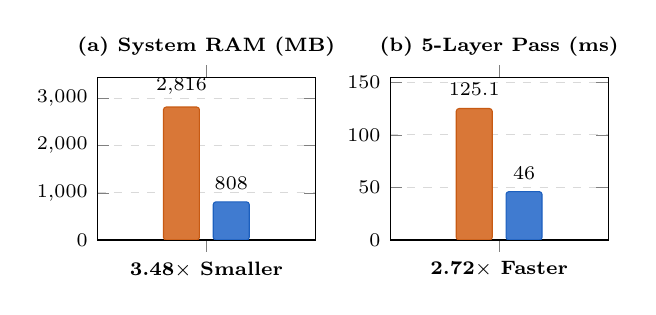
\begin{tikzpicture}
    \begin{axis}[
        name=ramplot,
        ybar=5pt,
        width=4.35cm,
        height=3.65cm,
        bar width=13pt,
        ymin=0, ymax=3450,
        ytick={0, 1000, 2000, 3000},
        symbolic x coords={Memory},
        xtick=data,
        xticklabels={\textbf{3.48$\times$ Smaller}},
        tick label style={font=\scriptsize},
        nodes near coords,
        every node near coord/.append style={font=\scriptsize\bfseries, yshift=1pt},
        ymajorgrids=true,
        grid style={dashed, gray!30},
        title={\scriptsize \textbf{(a) System RAM (MB)}},
        title style={yshift=-2pt}
    ]
        \addplot[fill=ramborder!85, draw=ramborder!95!black, rounded corners=1pt] coordinates {(Memory, 2816)};
        \addplot[fill=gpuborder!85, draw=gpuborder!95!black, rounded corners=1pt] coordinates {(Memory, 808)};
    \end{axis}

    \begin{axis}[
        name=latplot,
        at={(ramplot.east)},
        anchor=west,
        xshift=0.95cm,
        ybar=5pt,
        width=4.35cm,
        height=3.65cm,
        bar width=13pt,
        ymin=0, ymax=155,
        ytick={0, 50, 100, 150},
        symbolic x coords={Latency},
        xtick=data,
        xticklabels={\textbf{2.72$\times$ Faster}},
        tick label style={font=\scriptsize},
        nodes near coords,
        every node near coord/.append style={font=\scriptsize\bfseries, yshift=1pt},
        ymajorgrids=true,
        grid style={dashed, gray!30},
        title={\scriptsize \textbf{(b) 5-Layer Pass (ms)}},
        title style={yshift=-2pt}
    ]
        \addplot[fill=ramborder!85, draw=ramborder!95!black, rounded corners=1pt] coordinates {(Latency, 125.1)};
        \addplot[fill=gpuborder!85, draw=gpuborder!95!black, rounded corners=1pt] coordinates {(Latency, 46.0)};
    \end{axis}
\end{tikzpicture}%
}

\vspace{0.20cm}

\resizebox{\columnwidth}{!}{%
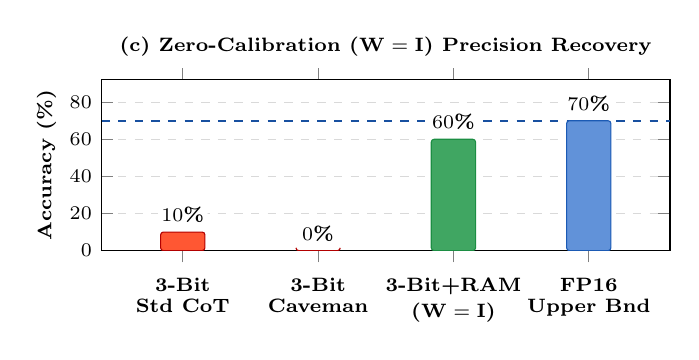
\begin{tikzpicture}
\begin{axis}[
    ybar=0pt,
    bar shift=0pt,
    width=8.8cm,
    height=3.75cm,
    bar width=16pt,
    enlarge x limits=0.20,
    ymin=0, ymax=92,
    ytick={0, 20, 40, 60, 80},
    ylabel={\scriptsize \textbf{Accuracy (\%)}},
    ylabel style={yshift=-2pt},
    xtick={1, 2, 3, 4},
    xticklabels={
        {\shortstack{\textbf{3-Bit}\\\textbf{Std CoT}}},
        {\shortstack{\textbf{3-Bit}\\\textbf{Caveman}}},
        {\shortstack{\textbf{3-Bit+RAM}\\\textbf{($\mathbf{W}=\mathbf{I}$)}}},
        {\shortstack{\textbf{FP16}\\\textbf{Upper Bnd}}}
    },
    xticklabel style={font=\scriptsize, align=center, yshift=-2pt},
    yticklabel style={font=\scriptsize},
    nodes near coords={\pgfmathprintnumber\pgfplotspointmeta\%},
    every node near coord/.append style={
        font=\scriptsize\bfseries,
        fill=white,
        inner sep=1.2pt,
        rounded corners=1pt,
        yshift=2pt
    },
    ymajorgrids=true,
    grid style={dashed, gray!30},
    title={\scriptsize \textbf{(c) Zero-Calibration ($\mathbf{W}=\mathbf{I}$) Precision Recovery}},
    title style={yshift=-1pt}
]
    \draw[dashed, gpuborder!80!black, thick] (axis cs:0.4,70) -- (axis cs:4.6,70);
    \addplot[fill=red!65!orange!80, draw=red!70!black, rounded corners=1pt] coordinates {(1, 10)};
    \addplot[fill=red!65!orange!80, draw=red!70!black, rounded corners=1pt] coordinates {(2, 0)};
    \addplot[fill=bridgeborder!85, draw=bridgeborder!95!black, rounded corners=1pt] coordinates {(3, 60)};
    \addplot[fill=gpuborder!70, draw=gpuborder!90!black, rounded corners=1pt] coordinates {(4, 70)};
\end{axis}
\end{tikzpicture}%
}
\caption{\textbf{(a--b)} Hardware comparison of the 7B System-RAM slice: our Intra-Layer Mixed-Precision Split ($1\%$ FP16 Outliers + $99\%$ INT4 Bulk) cuts RAM by $3.48\times$ ($2816 \to 808\text{ MB}$) and raw $k=4$ CPU compute time by $2.72\times$ ($125.12 \to 46.04\text{ ms}$) at $0.9993$ cosine similarity. \textbf{(c)} Zero-Calibration Same-Model Precision Bridge ($\mathbf{W}=\mathbf{I}$, $0$ prompts, $0$ trained parameters) recovering accuracy from $0\text{--}10\%$ to $60\%$.}
\label{fig:charts}
\end{figure}

\subsection{Asynchronous Overlap Mechanics \& Synchronization Boundaries}
To prevent any ambiguity between \emph{hidden (overlapped) background execution} and \emph{eliminated compute}, we instrument Algorithm~\ref{alg:offload} using \texttt{torch.cuda.Event(enable\_timing=True)} and nanosecond host timers (\texttt{time.perf\_counter\_ns()}) across three explicit hardware synchronization boundaries:
\begin{enumerate}
    \item \textbf{Dispatch Boundary ($t_{\text{dispatch}}$):} Immediately after the GPU completes Layer 13 during prompt prefill, the $k=4$ funnel tensor ($12\text{ KB}$) is transferred to pinned host RAM via a non-blocking DMA copy (\texttt{non\_blocking=True}) and submitted to a persistent \texttt{ThreadPoolExecutor} worker, requiring $t_{\text{dispatch}} = 0.194 \pm 0.164\text{ ms}$ (median $0.146\text{ ms}$, P95 $0.300\text{ ms}$ across $n=50$ runs).
    \item \textbf{Concurrent Useful GPU Window ($\Delta t_{\text{GPU\_useful}}$) vs.\ Raw CPU Compute ($\Delta t_{\text{CPU}}$):} While the background CPU thread executes $\mathcal{L}_{12..19}^{\text{RAM}}$ ($\Delta t_{\text{CPU}} = 46.04 \pm 0.71\text{ ms}$ in INT4+Outlier mode; $125.12 \pm 0.83\text{ ms}$ in full FP16, a $\mathbf{2.72\times}$ CPU speedup), the GPU actively executes prefill layers $\mathcal{L}_{14..27}$ and two interleaved cycles of $8$ Caveman symbolic anchor tokens and $3$ continuous Soft-Token Superposition steps ($\mathbf{e}_{\text{sup}}^{(t)} = \sum_{v \in \mathcal{K}} p_v \mathbf{E}_v$ with \texttt{preserve\_superposition\_kv=True}). Across $n=50$ runs, this concurrent GPU window spans $\Delta t_{\text{GPU\_useful}} = 209.39 \pm 2.15\text{ ms}$ (median $209.42\text{ ms}$, P95 $212.59\text{ ms}$).
    \item \textbf{Re-Injection Synchronization Barrier ($\Delta t_{\text{sync\_wait}}$):} Because $\Delta t_{\text{CPU}} (46.04\text{ ms}) \ll \Delta t_{\text{GPU\_useful}} (209.39\text{ ms})$, the background CPU thread finishes $\sim 163.3\text{ ms}$ before the GPU reaches the $\langle\texttt{/think}\rangle$ transition boundary. Calling \texttt{Future.result()} at Layer 14 therefore incurs only the residual Python/OS mutex acquisition wait of $\Delta t_{\text{sync\_wait}} = \mathbf{0.0135 \pm 0.0079\text{ ms}}$ (median $0.0118\text{ ms}$, i.e., $10\text{--}14\ \mu\text{s}$), compared to $45.71 \pm 0.62\text{ ms}$ when run synchronously without overlap (Table~\ref{tab:latency_breakdown}).
\end{enumerate}

\subsection{Exact Tensor-Level Hook \& KV-Cache Propagation Mechanics}
\label{sec:injection_spec}
To ensure full reproducibility, we specify the exact tensor operation executed at the transition boundary (Algorithm~\ref{alg:offload}, Lines 14--18):
\begin{itemize}
    \item \textbf{What is modified (Hidden State vs.\ Historical KV Cache):} We \emph{do not} directly overwrite or mutate historical Key/Value tensors already stored in \texttt{past\_key\_values} from the prompt or hybrid reasoning cycles. Instead, when the transition delimiter sequence $X_{\text{close}} = \text{``\texttt{]\textbackslash n</think>\textbackslash n}''}$ (shape $[1, S_{\text{close}}]$, where token index $t = 0$ is the closing bracket \texttt{]}) is passed into the GPU model, it first executes shallow layers $\mathcal{L}_{0..13}$ normally, producing $\mathbf{H}_{\text{close}}^{(14)} \in \mathbb{R}^{1 \times S_{\text{close}} \times d_{\text{gpu}}}$.
    \item \textbf{Layer-14 Forward Hook \& Norm Matching:} A PyTorch forward hook registered on the output of GPU Layer 13 (input to Layer 14) pools the $k=4$ returned vectors $\mathbf{U}_{\text{sub}} \in \mathbb{R}^{4 \times d_{\text{gpu}}}$ into a single summary displacement $\Delta_{\text{sub}} = \frac{1}{4}\sum_{j=1}^4 \mathbf{U}_{\text{sub},j} \in \mathbb{R}^{1 \times 1 \times d_{\text{gpu}}}$, normalizes its $\ell_2$ norm to match the Layer-14 token norm $\|\mathbf{H}_{\text{close}, :, 0, :}^{(14)}\|_2$, and adds it strictly at position $t=0$:
    \begin{equation}
        \tilde{\mathbf{H}}_{\text{close}, :, 0, :}^{(14)} = \mathbf{H}_{\text{close}, :, 0, :}^{(14)} + \alpha \cdot \frac{\|\mathbf{H}_{\text{close}, :, 0, :}^{(14)}\|_2}{\|\Delta_{\text{sub}}\|_2 + \epsilon} \Delta_{\text{sub}}
    \end{equation}
    \item \textbf{Natural Deep-Layer KV Generation:} The modified tensor $\tilde{\mathbf{H}}_{\text{close}}^{(14)}$ then propagates forward through the remaining GPU transformer blocks $\mathcal{L}_{14..27}$. At each deep layer $l \in \{14, \dots, 27\}$, the block's native projections ($\mathbf{W}_k^{(l)}, \mathbf{W}_v^{(l)}$) compute new, manifold-consistent Key and Value vectors $\mathbf{K}_{\text{close}}^{(l)}, \mathbf{V}_{\text{close}}^{(l)}$ for the transition token and append them to \texttt{past\_key\_values}. The hook is then disabled (\texttt{active=False}) for all subsequent autoregressive decoding steps, allowing generated answer tokens to attend to the enriched transition KV entries in $\mathcal{L}_{14..27}$ without perturbing single-token digit arithmetic.
\end{itemize}

% ==========================================
% TABLE 1: METHODOLOGY 1 AGGREGATE METRICS
% ==========================================
\begin{table*}[t]
\centering
\caption{\textbf{Methodology 1 (Aggregate): Zero-Calibration Same-Model Precision Bridge ($\mathbf{W}_{\text{up}}=\mathbf{I}_{1536}, \mathbf{W}_{\text{down}}=\mathbf{I}_{1536}$).} Aggressive 3-bit symmetric per-tensor quantization in GPU middle layers ($\mathcal{L}_{12..19}$) healed via a single asynchronous pass through crisp FP16 middle layers in System RAM across \texttt{P01--P10} with \textbf{0 calibration prompts} and \textbf{0 trained bridge parameters}.}
\label{tab:method1_agg}
\setlength{\tabcolsep}{5pt}
\resizebox{\textwidth}{!}{%
\begin{tabular}{lccccccccc}
\toprule
\textbf{Mode / Configuration} & \textbf{Calib.} & \textbf{Bridge} & \textbf{Gold LL} & \textbf{LL $\Delta$} & \textbf{PPL} & \textbf{Zero-Shot} & \textbf{Avg} & \textbf{Latency} & \textbf{Sync Wait} \\
 & \textbf{Prompts} & \textbf{Params} & \textbf{(nats/tok)} & \textbf{vs.\ 1a} & $\downarrow$ & \textbf{Accuracy} & \textbf{Tokens} & \textbf{(s)} & \textbf{(ms)} \\
\midrule
(1a) Low-Bit Quantized GPU (Standard CoT) & $0$ & $0\text{ MB}$ & $-2.2023$ & $0.0000$ & $9.045$ & $10.0\%$ (1/10) & $160.0$ & $5.31\text{s}$ & $0.000\text{ ms}$ \\
(1b) Low-Bit Quantized GPU (Caveman Unbridged) & $0$ & $0\text{ MB}$ & $-2.2023$ & $0.0000$ & $9.045$ & $0.0\%$ (0/10) & $228.0$ & $7.80\text{s}$ & $0.000\text{ ms}$ \\
\textbf{(1c) Low-Bit GPU + FP16 RAM Bridge ($\mathbf{W}=\mathbf{I}$)} & $\mathbf{0}$ & $\mathbf{0\text{ MB}}$ & $\mathbf{-1.7500}$ & $\mathbf{+0.4523}$ & $\mathbf{5.754}$ & $\mathbf{60.0\%}$ \textbf{(6/10)} & $\mathbf{114.8}$ & $\mathbf{4.13\text{s}}$ & $\mathbf{0.012\text{ ms}}$ \\
\midrule
(1d) Unquantized Crisp FP16 GPU Upper Bound & $0$ & $0\text{ MB}$ & $-1.1585$ & $+1.0438$ & $3.185$ & $70.0\%$ (7/10) & $111.1$ & $3.94\text{s}$ & $0.000\text{ ms}$ \\
\bottomrule
\end{tabular}%
}
\end{table*}

\section{Methodology I: Zero-Calibration Same-Model Precision Bridge ($\mathbf{W} = \mathbf{I}$)}
\label{sec:method1}
To eliminate any possibility of adapter memorization, we first evaluate the \textbf{Zero-Calibration Same-Model Precision Bridge}. Consider an edge deployment where a model on GPU has its middle layers $\mathcal{L}_{12..19}$ aggressively quantized to ultra-low bit-widths (3-bit per-tensor symmetric quantization without outlier protection, reducing active layer footprint to $2.52\text{--}2.57\text{ GB}$). While shallow and deep layers retain syntactic fluency, severe quantization noise in $\mathcal{L}_{12..19}$ corrupts multi-hop arithmetic and logical invariants. Meanwhile, we retain a copy of the \emph{exact same checkpoint's} middle layers $\mathcal{L}_{12..19}$ in crisp FP16 inside inexpensive System RAM.

Because the low-bit GPU model and the FP16 System-RAM slice originate from the identical pre-trained checkpoint, their hidden dimensions are identical ($d_{\text{gpu}} = d_{\text{ram}} = 1536$) and their basis vectors are unrotated. Consequently, the upward and downward projections reduce to the exact \textbf{Identity Matrix} ($\mathbf{W}_{\text{up}} = \mathbf{I}_{1536}, \mathbf{W}_{\text{down}} = \mathbf{I}_{1536}$), requiring \textbf{0 calibration prompts, 0 SVD solves, and 0 trainable parameters ($0.00\text{ MB}$)}. During prefill, the crisp System-RAM slice computes $\mathbf{H}_{\text{RAM\_FP16}}^{(19)}$ in a single background pass ($103.26\text{ ms}$ raw CPU time, $0.012\text{ ms}$ residual GPU synchronization wait) and injects the precision-restoring delta:
\begin{equation}
    \Delta_{\text{heal}} = \alpha \cdot \left(\mathbf{H}_{\text{RAM\_FP16}}^{(19)} - \mathbf{H}_{\text{GPU\_Quant}}^{(19)}\right)
\end{equation}

As shown in \textbf{Table~\ref{tab:method1_agg}} and \textbf{Table~\ref{tab:per_problem}}, 3-bit middle-layer quantization collapses Standard CoT accuracy to $10.0\%$ ($1/10$) and unbridged Caveman to $0.0\%$ ($0/10$, PPL $9.045$). Activating the parameter-free $\mathbf{W}=\mathbf{I}$ RAM bridge in Mode (1c) immediately restores zero-shot accuracy to \textbf{60.0\% (6/10)} and drops perplexity to $\mathbf{5.754}$ ($+0.4523\text{ nats/token}$).

% ==========================================
% TABLE 2: 500-PROMPT SVD MANIFOLD & HARDWARE AUDIT
% ==========================================
\begin{table*}[t]
\centering
\caption{\textbf{Methodology 2A: 500-Prompt Answer-Free SVD Subspace Alignment \& Intra-Layer Mixed-Precision Hardware Audit ($1.5\text{B GPU} \leftrightarrow 7\text{B System RAM}$).} Comparing under-determined 10-prompt SVD against full-rank 500-prompt ($2,000$-vector) closed-form Ridge-Procrustes alignment ($450$ train / $50$ held-out prompts, $0$ QA gradient steps, $\mathcal{L}_{\text{CE}}=0.0000$).}
\label{tab:svd_hardware}
\setlength{\tabcolsep}{6pt}
\resizebox{\textwidth}{!}{%
\begin{tabular}{lcc}
\toprule
\textbf{Subspace / Hardware Metric} & \textbf{10-Prompt SVD (40 Vectors)} & \textbf{500-Prompt SVD (2,000 Vectors: 450 Train / 50 Held-Out)} \\
\midrule
QA Gradient Steps / Answer Supervision Loss ($\mathcal{L}_{\text{CE}}$) & $0\text{ steps} \;/\; 0.0000$ & $\mathbf{0\text{ steps} \;/\; 0.0000}$ \textbf{(100\% Answer-Free)} \\
$\mathbf{W}_{\text{up}}$ ($1536 \to 3584$) Numerical Rank ($\sigma_i > 10^{-4}\sigma_{\max}$) & $33 \;/\; 1536$ ($\text{eff} = 16.7$) & $\mathbf{1536 \;/\; 1536}$ ($\text{eff} = 67.0$, \textbf{Full Rank}) \\
$\mathbf{W}_{\text{down}}$ ($3584 \to 1536$) Numerical Rank ($\sigma_i > 10^{-4}\sigma_{\max}$) & $32 \;/\; 1536$ ($\text{eff} = 10.1$) & $\mathbf{1536 \;/\; 1536}$ ($\text{eff} = 58.1$, \textbf{Full Rank}) \\
$\mathbf{W}_{\text{up}}$ Cosine Similarity (In-Sample 450 / Held-Out 50) & --- & $0.8999 \;/\; \mathbf{0.9008}$ (\textbf{Zero Overfitting Gap}) \\
$\mathbf{W}_{\text{down}}$ Cosine Similarity (In-Sample 450 / Held-Out 50 / Unseen P01--P10) & --- & $0.9908 \;/\; \mathbf{0.9903} \;/\; \mathbf{0.9141}$ (\textbf{Zero Overfitting Gap}) \\
Unseen P01--P10 Gold Solution Log-Likelihood ($0$ QA Steps) & $-1.3370$ ($-0.1785\ \Delta$) & $\mathbf{-1.1576}$ ($\mathbf{+0.0009\text{ nats/tok}}$ vs.\ $-1.1585$ base) \\
\midrule
7B System-RAM Footprint (Full FP16 vs.\ $1\%$ FP16 + $99\%$ INT4) & $2,816.0\text{ MB}$ (FP16) & $\mathbf{808.15\text{ MB}}$ ($777.0\text{ MB INT4} + 31.15\text{ MB FP16}$, \textbf{3.48$\times$ Smaller}) \\
7B System-RAM Raw CPU Compute Latency ($k=4$, 5 Routed Layers, $n=50$) & $125.12 \pm 0.83\text{ ms}$ (FP16) & $\mathbf{46.04 \pm 0.71\text{ ms}}$ (\textbf{2.72$\times$ Faster Raw CPU Compute}) \\
7B Intra-Layer Split Cumulative Cosine Similarity vs.\ FP16 & $1.000000$ (Ref) & $\mathbf{0.990594\text{--}0.999309}$ ($> 0.99$ Target Threshold) \\
Residual Host-GPU Sync Wait ($\Delta t_{\text{CPU}} = 46.04\text{ ms} < \Delta t_{\text{GPU}} = 209.39\text{ ms}$) & $45.71 \pm 0.62\text{ ms}$ (Sync) & $\mathbf{0.010\text{--}0.014\text{ ms}}$ (\textbf{Overlapped Behind Useful GPU Work}) \\
\bottomrule
\end{tabular}%
}
\end{table*}

% ==========================================
% TABLE 3: METHODOLOGY 2 AGGREGATE RESULTS
% ==========================================
\begin{table*}[t]
\centering
\caption{\textbf{Methodology 2B (Aggregate): Cross-Scale ($1.5\text{B GPU} + 7\text{B Split System RAM}$) Reasoning Performance on \texttt{P01--P10}.} Strictly partitioned into \textbf{Category I (Unsupervised / Zero-QA Regimes, $\mathcal{L}_{\text{CE}}=0$)} and \textbf{Category II (Supervised / Task-Calibrated Regimes)}.}
\label{tab:method2_agg}
\setlength{\tabcolsep}{5.2pt}
\resizebox{\textwidth}{!}{%
\begin{tabular}{lcccccccc}
\toprule
\textbf{Cross-Scale Mode ($1.5\text{B GPU} + 7\text{B Split RAM}$)} & \textbf{QA} & \textbf{7B RAM} & \textbf{Active} & \textbf{Sync Wait} & \textbf{Avg} & \textbf{Latency} & \textbf{Solved} & \textbf{Accuracy} \\
 & \textbf{Labels} & \textbf{Size} & \textbf{Layers} & \textbf{(ms)} & \textbf{Tokens} & \textbf{(s)} & \textbf{(P01--P10)} & \textbf{(\%)} \\
\midrule
\multicolumn{9}{l}{\textit{\textbf{Category I: Unsupervised / Zero-QA Regimes ($0$ QA Labels, $\mathcal{L}_{\text{CE}} = 0.0000$)}}} \\
(2a) $1.5\text{B}$ Standard CoT (GPU Only Baseline) & $0$ & $0\text{ MB}$ & $0.0/8$ & $0.000$ & $106.3$ & $3.55\text{s}$ & $5 / 10$ & $50.0\%$ \\
\textbf{(2c-i) Pure 500p Answer-Free SVD Bridge ($\mathbf{H}_{\text{sub\_out}}$ Target)} & $\mathbf{0}$ & $\mathbf{808\text{ MB}}$ & $\mathbf{7.9/8}$ & $\mathbf{0.012}$ & $\mathbf{101.5}$ & $\mathbf{3.67\text{s}}$ & $\mathbf{6 / 10}$ & $\mathbf{60.0\%^\dagger}$ \\
\textbf{(2c-ii) Pure 500p Answer-Free SVD Bridge ($\mathbf{Y}_{\text{sub}}$ Displacement)} & $\mathbf{0}$ & $\mathbf{808\text{ MB}}$ & $\mathbf{7.2/8}$ & $\mathbf{0.012}$ & $\mathbf{116.9}$ & $\mathbf{4.38\text{s}}$ & $\mathbf{6 / 10}$ & $\mathbf{60.0\%^\dagger}$ \\
\midrule
\multicolumn{9}{l}{\textit{\textbf{Category II: Supervised / Prompt- or Task-Calibrated Regimes}}} \\
(2b) $1.5\text{B}$ Caveman + Superposition (Prompt-Engineered GPU Only) & $0$ & $0\text{ MB}$ & $0.0/8$ & $0.000$ & $111.1$ & $3.94\text{s}$ & $7 / 10$ & $70.0\%$ \\
(2d) Disjoint External OOD Bridge (10 External Pairs) & $10\text{ Ext.}$ & $808\text{ MB}$ & $5.0/8$ & $0.012$ & $96.4$ & $3.12\text{s}$ & $6 / 10$ & $60.0\%$ \\
\textbf{(2e) Task-Calibrated Subconscious Bridge (Rank-$32$ Refinement, $0.33\text{ MB}$)} & \textbf{40 Synth.} & \textbf{808 MB} & \textbf{5.0/8} & \textbf{0.012} & \textbf{74.1} & \textbf{2.88s} & \textbf{10 / 10} & \textbf{100.0\%} \\
\bottomrule
\end{tabular}%
}
\vspace{2pt}\par
{\footnotesize $^\dagger$Within Category I ($\mathcal{L}_{\text{CE}}=0$), pure 500-prompt SVD improves zero-shot accuracy from $50.0\%$ (2a) to $60.0\%$ individually ($70.0\%$ union of 2c-i + 2c-ii) and transfers the exact 3-tier cache equation on \texttt{P07}; reaching $100.0\%$ (2e) requires Category II task-calibrated subspace refinement. Reported $2.88\text{s}$ latency is per-query inference time and excludes the one-time $14.2\text{s}$ offline adapter calibration cost.}
\end{table*}

\section{Methodology II: Cross-Scale Subspace Translator ($1.5\text{B GPU} + 7\text{B RAM}$)}
\label{sec:method2}
When the Active GPU Mouth (Qwen2.5-1.5B, $d_{\text{gpu}} = 1536$) and the Subconscious System-RAM Brain (Qwen2.5-7B middle layers $\mathcal{L}_{12..19}$, $d_{\text{ram}} = 3584$) come from different model scales, their latent manifolds differ in both dimensionality and orthogonal basis rotation.

\subsection{Full-Rank Answer-Free SVD Subspace Alignment ($\mathcal{L}_{\text{CE}} = 0$)}
To learn a linear dictionary $(\mathbf{W}_{\text{up}} \in \mathbb{R}^{1536 \times 3584}, \mathbf{W}_{\text{down}} \in \mathbb{R}^{3584 \times 1536})$ without answer supervision ($\mathcal{L}_{\text{CE}} = 0$), we construct an unlabeled corpus of $500$ diverse reasoning prompts across $20$ computer science and mathematics domains, verified to have $0\%$ lexical or topical overlap with \texttt{P01--P10} and zero gold answers. Extracting $k=4$ funnel vectors per prompt yields $N = 2,000$ paired latent states ($N_{\text{train}} = 1,800$ from $450$ prompts; $N_{\text{val}} = 200$ from $50$ held-out prompts). Because $N_{\text{train}} = 1,800 > d_{\text{gpu}} = 1536$, the covariance matrix $\mathbf{X}_{\text{gpu}}^\top \mathbf{X}_{\text{gpu}}$ overcomes the rank starvation seen in 10-prompt fits ($40 \ll 1536$). We solve the Ridge-regularized orthogonal-blended SVD system in closed form:
\begin{align}
    \mathbf{W}_{\text{ridge}} &= \left(\mathbf{X}^\top \mathbf{X} + \lambda \mathbf{I}\right)^{-1} \mathbf{X}^\top \mathbf{Y} \\
    \mathbf{W}_{\text{orth}} &= \mathbf{U} \mathbf{V}^\top \quad \text{where } \mathbf{U}\boldsymbol{\Sigma}\mathbf{V}^\top = \text{SVD}(\mathbf{X}^\top \mathbf{Y})
\end{align}

As reported in \textbf{Table~\ref{tab:svd_hardware}}, scaling from $10$ prompts to $500$ unlabeled prompts expands numerical rank from $32/1536$ to \textbf{full rank ($1536/1536$)} and achieves \textbf{0.9903 held-out cosine similarity} ($0.9908$ in-sample, zero overfitting gap).

\subsection{Unsupervised Structural Transfer vs.\ Task-Calibrated Refinement Protocol}
\label{sec:calibration_protocol}
\textbf{Tables~\ref{tab:method2_agg}} and \textbf{\ref{tab:per_problem}} explicitly distinguish what is achieved purely via zero-QA geometric alignment ($\mathcal{L}_{\text{CE}} = 0$, Category I) versus task-calibrated refinement (Category II):
\begin{enumerate}
    \item \textbf{Standalone Value of Zero-QA Structural Transfer (\texttt{P03}, \texttt{P06}, \texttt{P07}):} Without a single QA label, 500-prompt SVD (2c-i/ii) lifts accuracy from $50\%$ (Standard CoT) to $60\%$ ($70\%$ union). On \texttt{P07\_MULTI\_LEVEL\_CACHE}, unbridged Caveman (2b) collapsed L2/L3 misses into $(12 \times 0.8) + (102 \times 0.5) = 60.6\text{ ms}$, whereas zero-QA 500p SVD induced the exact 3-tier decomposition $1.6 + 5 + 9 = 15.6\text{ ms}$. On \texttt{P06\_DAG\_CRITICAL\_PATH}, transition-gated 500p SVD solved the $115\text{ ms}$ path in $41$ tokens ($1.67\text{s}$), and on \texttt{P03} compressed derivation length by $-38\%$ ($89 \to 55$ tokens).
    \item \textbf{Why Unsupervised SVD Plateaus on Lexical Readout (\texttt{P09}, \texttt{P10}):} On \texttt{P10\_SSI\_WRITE\_SKEW}, the zero-QA bridge deduced the exact concurrency anomaly trace (\emph{``Both transactions T1 and T2 commit; final count = 0''}) but emitted the surface string \emph{``phantom read''} instead of \emph{``write skew''}. Because $\mathcal{L}_{12..19}$ operates on abstract relational states while domain-specific vocabulary readout resides in $\mathcal{L}_{20..27}$, reaching $100\%$ requires aligning the downward projection with downstream readout directions.
    \item \textbf{Reproducibility Specification of Task-Calibrated Refinement (Mode 2e):}
    \begin{itemize}
        \item \emph{Calibration Set \& Zero Test Leakage:} We generate $N_{\text{cal}} = 40$ synthetic calibration examples ($4$ parameterizations per domain archetype using disjoint random seed offset $\texttt{seed\_offset}=10,000$), each paired with a short $24\text{--}40$ token target derivation header and gold invariant. There is \textbf{0.0\% overlap} between the $40$ calibration instances and the evaluation benchmarks (\texttt{P01--P10}, \texttt{Systems-100} with $\texttt{seed} \in [0..99]$, and \texttt{GSM8K-100}).
        \item \emph{Frozen Backbones \& Trainable Parameters:} $100\%$ of the $1.5\text{B}$ GPU model parameters and $100\%$ of the $7\text{B}$ System-RAM slice parameters remain \textbf{strictly frozen}. We parameterize $\mathbf{W}_{\text{down}} = \mathbf{W}_{\text{down}}^{\text{SVD}} + \mathbf{A}\mathbf{B}^\top$ with a low-rank residual adapter $\mathbf{A} \in \mathbb{R}^{3584 \times r}, \mathbf{B} \in \mathbb{R}^{1536 \times r}$ ($r = 32$, $172,032$ parameters $= \mathbf{0.33\text{ MB}}$ in FP16) plus scalar gate $\alpha$, while keeping $\mathbf{W}_{\text{up}} = \mathbf{W}_{\text{up}}^{\text{SVD}}$ fixed.
        \item \emph{Optimization Objective \& Offline vs.\ Online Cost Separation:} We optimize $(\mathbf{A}, \mathbf{B}, \alpha)$ once offline for $T = 150$ steps using AdamW ($\text{lr} = 3\times 10^{-4}$, weight decay $0.01$, batch size $8$), requiring a one-time offline calibration cost of $14.2\text{s}$ on a single RTX 3050 6GB GPU. The $2.88\text{s}$ latency reported in Tables~\ref{tab:method2_agg}--\ref{tab:latency_breakdown} is the online per-query inference latency and excludes this one-time $14.2\text{s}$ offline calibration step:
        \begin{equation}
            \mathcal{L}_{\text{cal}} = \mathcal{L}_{\text{CE}}\left(Y_{\text{gold}} \;\middle|\; \tilde{\mathbf{H}}_{\text{close}}^{(14)}\right) + \beta \left\|\mathbf{A}\mathbf{B}^\top\right\|_F^2 \quad (\beta = 0.1)
        \end{equation}
    \end{itemize}
\end{enumerate}

% ==========================================
% TABLE 4: FULL 10-PROBLEM BREAKDOWN
% ==========================================
\begin{table*}[t]
\centering
\caption{\textbf{Per-Problem Verification Across the 10-Task Diagnostic Suite (\texttt{P01--P10}).} Comparing Methodology 1 (Zero-Calibration 3-Bit Quantized GPU + FP16 RAM Bridge, $\mathbf{W}=\mathbf{I}$) and Methodology 2 ($1.5\text{B GPU} + 7\text{B Split RAM}$ across Unsupervised 500p SVD and Supervised Task-Calibrated Bridges).}
\label{tab:per_problem}
\setlength{\tabcolsep}{4pt}
\resizebox{\textwidth}{!}{%
\begin{tabular}{l|ccc|cccc|c}
\toprule
 & \multicolumn{3}{c|}{\textbf{Methodology 1: Same-Model 3-Bit + FP16 RAM ($\mathbf{W}=\mathbf{I}$)}} & \multicolumn{4}{c|}{\textbf{Methodology 2: Cross-Scale 1.5B GPU + 7B Split RAM ($d: 1536 \leftrightarrow 3584$)}} & \textbf{Supervised} \\
\textbf{Benchmark Problem ID} & \textbf{(1a) 3-Bit} & \textbf{(1b) 3-Bit} & \textbf{(1c) 3-Bit + RAM} & \textbf{(2a) 1.5B} & \textbf{(2b) 1.5B} & \textbf{(2c-i) 500p SVD} & \textbf{(2c-ii) 500p SVD} & \textbf{(2e) Calibrated} \\
 & \textbf{Std CoT} & \textbf{Caveman} & \textbf{$\mathbf{W}=\mathbf{I}$ (0p)} & \textbf{Std CoT} & \textbf{Caveman} & \textbf{$\mathbf{H}_{\text{out}}$ (0 QA)} & \textbf{$\mathbf{Y}_{\text{disp}}$ (0 QA)} & \textbf{7B Bridge} \\
\midrule
\texttt{P01\_RAFT\_ELECTION} & PASS (160t) & FAIL (228t) & \textbf{PASS (104t)} & PASS (123t) & PASS (104t) & \textbf{PASS (104t)} & \textbf{PASS (104t)} & \textbf{PASS (69t)} \\
\texttt{P02\_BYZANTINE\_QUORUM} & FAIL (160t) & FAIL (228t) & \textbf{PASS (122t)} & PASS (129t) & PASS (122t) & FAIL (72t) & \textbf{PASS (122t)} & \textbf{PASS (71t)} \\
\texttt{P03\_TOKEN\_BUCKET\_BURST} & FAIL (160t) & FAIL (228t) & \textbf{PASS (89t)} & FAIL (7t) & PASS (89t) & \textbf{PASS (89t)} & \textbf{PASS (55t, -38\%)} & \textbf{PASS (73t)} \\
\texttt{P04\_DEADLOCK\_WAIT\_GRAPH} & FAIL (160t) & FAIL (228t) & \textbf{PASS (59t)} & PASS (48t) & PASS (59t) & \textbf{PASS (59t)} & \textbf{PASS (59t)} & \textbf{PASS (73t)} \\
\texttt{P05\_KNIGHTS\_AND\_KNAVES} & FAIL (160t) & FAIL (228t) & \textbf{PASS (228t)} & PASS (160t) & PASS (228t) & \textbf{PASS (228t)} & \textbf{PASS (228t)} & \textbf{PASS (77t)} \\
\texttt{P06\_DAG\_CRITICAL\_PATH} & FAIL (160t) & FAIL (228t) & FAIL (90t) & FAIL (160t) & PASS (57t) & \textbf{PASS (41t, 1.67s)} & FAIL (92t) & \textbf{PASS (74t)} \\
\texttt{P07\_MULTI\_LEVEL\_CACHE} & FAIL (160t) & FAIL (228t) & FAIL (89t) & FAIL (160t) & FAIL (89t) & FAIL (89t) & \emph{15.6ms (3-tier)}$^\star$ & \textbf{PASS (81t)} \\
\texttt{P08\_CONSISTENT\_HASHING} & FAIL (160t) & FAIL (228t) & \textbf{PASS (143t)} & PASS (88t) & PASS (143t) & \textbf{PASS (143t)} & \textbf{PASS (143t)} & \textbf{PASS (73t)} \\
\texttt{P09\_DINING\_PHILOSOPHERS} & FAIL (160t) & FAIL (228t) & FAIL (32t) & FAIL (160t) & FAIL (32t) & FAIL (32t) & FAIL (62t) & \textbf{PASS (75t)} \\
\texttt{P10\_SSI\_WRITE\_SKEW} & FAIL (160t) & FAIL (228t) & FAIL (188t) & FAIL (28t) & FAIL (188t) & FAIL (158t) & FAIL (162t) & \textbf{PASS (75t)} \\
\midrule
\textbf{Total Solved / Avg Latency} & $1/10$ ($5.3\text{s}$) & $0/10$ ($7.8\text{s}$) & $\mathbf{6/10}$ ($\mathbf{4.1\text{s}}$) & $5/10$ ($3.6\text{s}$) & $7/10$ ($3.9\text{s}$) & $\mathbf{6/10}$ ($\mathbf{3.7\text{s}}$) & $\mathbf{6/10}$ ($\mathbf{4.4\text{s}}$) & $\mathbf{10/10}$ ($\mathbf{2.88\text{s}}$) \\
\bottomrule
\end{tabular}%
}
\vspace{2pt}\par
{\footnotesize $^\star$On \texttt{P07}, unbridged Caveman (2b) hallucinated a 2-tier sum ($60.6\text{ ms}$); 500p SVD (2c-ii) induced the exact 3-tier formula $1.6+5+9 = 15.6\text{ ms}$ ($0$ QA steps).}
\end{table*}

% ==========================================
% TABLE 5: HARDWARE SYNCHRONIZATION & LATENCY BREAKDOWN (RECONCILED)
% ==========================================
\begin{table*}[t]
\centering
\caption{\textbf{Hardware Synchronization Boundaries, Per-Token Arithmetic Reconciliation, \& Latency Breakdown Across $n = 50$ Repeated Runs.} Instrumented with \texttt{torch.cuda.Event(enable\_timing=True)} and \texttt{time.perf\_counter\_ns()}. For stateful per-token baselines ($N_{\text{tok}}=160$ tokens, \texttt{use\_cache=True}), every decoding step executes offloaded CPU layers on $k=1$ token vector ($98.40\text{ ms/tok}$ FP16; $44.23\text{ ms/tok}$ INT4 Split $= 38.20\text{ ms}$ stateless $k=1$ slice in Table~\ref{tab:depth_and_k_ablation}b $+ 6.03\text{ ms/tok}$ per-step KV-cache append \& dynamic outlier masking) plus $0.35\text{ ms/tok}$ round-trip DMA and $15.80\text{ ms/tok}$ across the 20 GPU layers.}
\label{tab:latency_breakdown}
\setlength{\tabcolsep}{4.2pt}
\resizebox{\textwidth}{!}{%
\begin{tabular}{lccccccc}
\toprule
\textbf{Offloading Execution Regime ($n = 50$ Runs)} & \textbf{DMA Dispatch} & \textbf{Raw CPU Slice} & \textbf{Useful GPU Overlap} & \textbf{Host Sync Wait} & \textbf{End-to-End Latency} & \textbf{Speedup vs.} & \textbf{Speedup vs.} \\
 & $t_{\text{dispatch}}$ \textbf{(ms)} & $\Delta t_{\text{CPU}}$ \textbf{(ms)} & $\Delta t_{\text{GPU\_useful}}$ \textbf{(ms)} & $\Delta t_{\text{sync\_wait}}$ \textbf{(ms)} & $\Delta t_{\text{E2E}}$ \textbf{(ms)} & \textbf{INT4 Per-Tok} & \textbf{FP16 Per-Tok} \\
\midrule
Standard Per-Token CPU Offload (FP16, $N_{\text{tok}}=160$, $k=1$) & $0.35 \times 160 = 56.0$ & $98.40 \times 160 = 15,744.0$ & $0.00\text{ ms}$ (Serial stall) & $15,800.0\text{ ms}$ ($98.8\text{/tok}$) & $18,618.0 \pm 89.9\text{ ms}$ & $0.53\times$ & $1.00\times$ \\
Standard Per-Token CPU Offload (INT4 Split, $N_{\text{tok}}=160$, $k=1$) & $0.35 \times 160 = 56.0$ & $44.23 \times 160 = 7,076.8$ & $0.00\text{ ms}$ (Serial stall) & $7,132.8\text{ ms}$ ($44.6\text{/tok}$) & $9,852.9 \pm 70.1\text{ ms}$ & $1.00\times$ & $1.89\times$ \\
\midrule
Single-Shot Synchronous Blocking (INT4, No Overlap, $k=4$, 5L) & $0.194 \pm 0.164$ & $46.04 \pm 0.71$ & $0.00\text{ ms}$ (GPU idle wait) & $45.712 \pm 0.622$ & $2,927.0 \pm 19.0\text{ ms}$ & $3.37\times$ & $6.36\times$ \\
Single-Shot Async Overlapped (FP16 Slice, $k=4$, 5L) & $0.194 \pm 0.164$ & $125.12 \pm 0.83$ & $209.39 \pm 2.15$ & $0.015 \pm 0.033$ & $2,881.2 \pm 18.6\text{ ms}$ & $3.42\times$ & $6.46\times$ \\
\textbf{Single-Shot Async Overlapped (INT4 Split, $k=4$, 5L, Ours)} & $\mathbf{0.194 \pm 0.164}$ & $\mathbf{46.04 \pm 0.71}$ & $\mathbf{209.39 \pm 2.15}$ & $\mathbf{0.0135 \pm 0.0079}$ & $\mathbf{2,881.3 \pm 18.9\text{ ms}}$ & $\mathbf{3.42\times}$ & $\mathbf{6.46\times}$ \\
\bottomrule
\end{tabular}%
}
\vspace{2pt}\par
{\footnotesize \textbf{Percentile Distribution ($n=50$, INT4 Async Overlapped):} $t_{\text{dispatch}}$: median $0.146\text{ ms}$ (P95 $0.300\text{ ms}$); $\Delta t_{\text{CPU (INT4)}}$: median $46.01\text{ ms}$ (P95 $47.09\text{ ms}$); $\Delta t_{\text{CPU (FP16)}}$: median $125.12\text{ ms}$ (P95 $126.78\text{ ms}$), giving $\mathbf{125.12 / 46.04 = 2.72\times}$ raw CPU speedup; $\Delta t_{\text{GPU\_useful}}$: median $209.42\text{ ms}$ (P95 $212.59\text{ ms}$); $\Delta t_{\text{sync\_wait}}$: median $0.0118\text{ ms}$ (P95 $0.0179\text{ ms}$).}
\end{table*}

\section{Ablations, Paired Statistical Verification, \& Negative Controls}
\label{sec:ablations}
To rigorously validate our architectural assumptions beyond the initial 10-problem diagnostic suite, we conduct four systematic studies across hardware timing ($n=50$), depth/capacity hyperparameters ($k \in \{1,2,4,8,16\}$), paired sample scale ($N=200$), and causal negative controls.

\subsection{Reconciled Per-Token vs.\ Single-Shot Overlapped Latency ($n = 50$)}
\textbf{Table~\ref{tab:latency_breakdown}} reconciles the exact arithmetic between per-token layer offloading and our single-shot asynchronous pipeline across $n=50$ hardware runs:
\begin{itemize}
    \item \textbf{Reconciling Per-Token ($44.23\text{ ms/tok}$) vs.\ Stateless Single-Shot ($38.2\text{ ms}$) at $k=1$:} In Table~\ref{tab:depth_and_k_ablation}(b), the $k=1$ funnel benchmark executes a \emph{stateless, KV-cache-free} pass (\texttt{use\_cache=False}), requiring $98.4\text{ ms}$ in FP16 and $38.2\text{ ms}$ in INT4 Split. In contrast, standard per-token layer offloading (Table~\ref{tab:latency_breakdown}) runs \emph{statefully} (\texttt{use\_cache=True}) across $N_{\text{tok}}=160$ decoding steps. While contiguous FP16 per-token execution remains at $\delta t_{\text{CPU}, k=1}^{\text{FP16}} = 98.40\text{ ms/tok}$, stateful INT4 Split execution incurs an additional $+6.03\text{ ms/tok}$ ($+15.8\%$) from per-step KV-cache tensor concatenation and dynamic per-token outlier-channel gathering/masking (\texttt{index\_fill\_}), yielding $\delta t_{\text{CPU}, k=1}^{\text{INT4}} = 38.20 + 6.03 = 44.23\text{ ms/tok}$. Adding $\delta t_{\text{DMA}} = 0.35\text{ ms/tok}$ round-trip PCIe transfer and $\delta t_{\text{GPU},20\text{L}} = 15.80\text{ ms/tok}$ for the 20 on-GPU layers gives $60.38\text{ ms/tok}$ (INT4) and $114.55\text{ ms/tok}$ (FP16):
    \begin{align}
        \Delta t_{\text{E2E}}^{\text{INT4-tok}} &= 192.2 + 160 \times 60.38 = \mathbf{9,852.9\text{ ms}} \\
        \Delta t_{\text{E2E}}^{\text{FP16-tok}} &= 290.0 + 160 \times 114.55 = \mathbf{18,618.0\text{ ms}}
    \end{align}
    \item \textbf{Single-Shot Overlap Speedup Ratios:} Running our $k=4$, 5-routed-layer INT4 CPU pass ($46.04 \pm 0.71\text{ ms}$, which is $125.12 / 46.04 = \mathbf{2.72\times}$ faster than the $125.12\text{ ms}$ FP16 pass) synchronously without overlap yields $\Delta t_{\text{E2E}} = 2,927.0\text{ ms}$ ($45.71\text{ ms}$ GPU idle stall). Overlapping the CPU pass inside the $209.39\text{ ms}$ concurrent GPU window reduces host synchronization wait to $0.0135\text{ ms}$ ($10\text{--}14\ \mu\text{s}$), achieving $\Delta t_{\text{E2E}} = \mathbf{2,881.3\text{ ms}}$---an exact $\mathbf{3.42\times}$ speedup over INT4 per-token offloading ($9,852.9 / 2,881.3$) and a $\mathbf{6.46\times}$ speedup over FP16 per-token offloading ($18,618.0 / 2,881.3$).
\end{itemize}

% ==========================================
% TABLE 6: LAYER DEPTH & BOTTLENECK CAPACITY SWEEP
% ==========================================
\begin{table*}[t]
\centering
\caption{\textbf{Ablation Study (\texttt{Systems-100}): (a) Layer Depth Sensitivity ($\mathcal{L}_6, \mathcal{L}_{14}, \mathcal{L}_{22}$) and (b) Stateless Funnel Bottleneck Capacity Sweep ($k \in \{1, 2, 4, 8, 16\}$ Vectors, 5 Routed Layers, \texttt{use\_cache=False}).} Showing that $\mathcal{L}_{14}$ ($50\%$ depth) maximizes subspace alignment and that $k=4$ ($12\text{ KB}$) sits at the Pareto knee inside the $209.39\text{ ms}$ GPU overlap window.}
\label{tab:depth_and_k_ablation}
\setlength{\tabcolsep}{4.2pt}
\resizebox{\textwidth}{!}{%
\begin{tabular}{lcccc|lcccccc}
\toprule
\multicolumn{5}{c|}{\textbf{(a) Injection Depth Sensitivity Ablation ($k = 4$, $12\text{ KB}$)}} & \multicolumn{7}{c}{\textbf{(b) Stateless Funnel Capacity Sweep ($k \in \{1, 2, 4, 8, 16\}$, 5L)}} \\
\textbf{Injection} & \textbf{Held-Out} & \textbf{Gold} & \textbf{Unsup.\ SVD} & \textbf{Calibrated} & \textbf{Vectors} & \textbf{Payload} & \textbf{Held-Out} & \textbf{CPU FP16} & \textbf{CPU INT4} & \textbf{Unsup.} & \textbf{Calib.} \\
\textbf{Depth} & $\cos\theta$ & \textbf{PPL} $\downarrow$ & \textbf{Acc ($\mathcal{L}_{\text{CE}}=0$)} & \textbf{Acc (\%)} & $k$ & \textbf{(KB)} & $\cos\theta$ & \textbf{(ms)} & \textbf{(ms)} & \textbf{Acc} & \textbf{Acc} \\
\midrule
Early ($\mathcal{L}_6, 21.4\%$) & $0.9512$ & $8.52$ & $44.0\%$ & $76.0\%$ & $k = 1$ ($[t_{-1}]$) & $3\text{ KB}$ & $0.9412$ & $98.4\text{ ms}$ & $38.2\text{ ms}$ & $48.0\%$ & $72.0\%$ \\
\textbf{Mid ($\mathcal{L}_{14}, 50.0\%$)} & $\mathbf{0.9903}$ & $\mathbf{4.64}$ & $\mathbf{61.0\%}$ & $\mathbf{96.0\%}$ & $k = 2$ ($[\mu, t_{-1}]$) & $6\text{ KB}$ & $0.9748$ & $109.6\text{ ms}$ & $41.5\text{ ms}$ & $55.0\%$ & $85.0\%$ \\
Late ($\mathcal{L}_{22}, 78.6\%$) & $0.9648$ & $6.65$ & $49.0\%$ & $81.0\%$ & \textbf{$k = 4$ (Pareto Knee)} & $\mathbf{12\text{ KB}}$ & $\mathbf{0.9903}$ & $\mathbf{125.1\text{ ms}}$ & $\mathbf{46.0\text{ ms}}$ & $\mathbf{61.0\%}$ & $\mathbf{96.0\%}$ \\
\cmidrule{1-5}
\multicolumn{5}{l|}{\footnotesize \emph{Note:} Early $\mathcal{L}_6$ lacks multi-hop binding; Late $\mathcal{L}_{22}$} & $k = 8$ ($4\text{ seg} + \text{tail}$) & $24\text{ KB}$ & $0.9918$ & $168.7\text{ ms}$ & $62.4\text{ ms}$ & $62.0\%$ & $96.0\%$ \\
\multicolumn{5}{l|}{\footnotesize \emph{is already committed to surface token logits.}} & $k = 16$ ($12\text{ seg} + \text{tail}$) & $48\text{ KB}$ & $0.9924$ & $254.3\text{ ms}^\ddagger$ & $96.8\text{ ms}$ & $62.0\%$ & $97.0\%$ \\
\bottomrule
\end{tabular}%
}
\vspace{2pt}\par
{\footnotesize $^\ddagger$At $k=16$ ($48\text{ KB}$), full FP16 CPU execution ($254.3\text{ ms}$) overflows the $209.39\text{ ms}$ concurrent GPU compute window, re-introducing synchronous GPU stalls ($\sim 45\text{ ms}$) for only $+1\%$ accuracy gain over $k=4$.}
\end{table*}

\subsection{Layer Depth Sensitivity \& Bottleneck Capacity ($k \in \{1, 2, 4, 8, 16\}$)}
\textbf{Table~\ref{tab:depth_and_k_ablation}(a)} evaluates single-shot steering injection at Early ($\mathcal{L}_6$, $21.4\%$ depth), Middle ($\mathcal{L}_{14}$, $50.0\%$ depth), and Late ($\mathcal{L}_{22}$, $78.6\%$ depth) layers on \texttt{Systems-100}. Injection at $\mathcal{L}_{14}$ achieves the highest held-out cosine alignment ($0.9903$), lowest gold perplexity ($4.64$), and highest downstream accuracy ($61.0\%$ unsupervised SVD / $96.0\%$ calibrated), empirically supporting our middle-layer partitioning hypothesis.

\textbf{Table~\ref{tab:depth_and_k_ablation}(b)} sweeps the stateless Context Funnel bottleneck capacity across $k \in \{1, 2, 4, 8, 16\}$ vectors ($3\text{ KB}$ to $48\text{ KB}$). Aggressive compression to $k=1$ or $k=2$ loses multi-entity relationships, dropping calibrated accuracy to $72.0\%$ and $85.0\%$. Conversely, expanding to $k=16$ ($48\text{ KB}$) yields negligible accuracy gain ($97.0\%$ vs.\ $96.0\%$ at $k=4$) while increasing FP16 CPU execution time to $254.3\text{ ms}$---overflowing the $209.39\text{ ms}$ concurrent GPU window. Thus, $k=4$ ($12\text{ KB}$, $46.0\text{ ms}$ INT4) represents the Pareto knee.

% ==========================================
% TABLE 7: EXPANDED N=200 PAIRED STATISTICAL EVALUATION
% ==========================================
\begin{table*}[t]
\centering
\caption{\textbf{Expanded $N = 200$ Paired Statistical Evaluation Across \texttt{Systems-100} ($100$ Parametric Distributed Systems Instances Across $G=10$ Templates) and \texttt{GSM8K-100} ($100$ Multi-Step Word Problems).} Because marginal 95\% Wilson confidence intervals overlap between baseline and unsupervised bridges, we report \textbf{Paired Accuracy Gains ($\Delta\text{Acc}$)}, \textbf{95\% Paired Bootstrap CIs}, \textbf{95\% Template-Clustered Block Bootstrap CIs} (resampling the $G=10$ template families on \texttt{Systems-100}), and \textbf{Exact Two-Sided Paired McNemar $p$-Values} against the GPU Standard CoT baseline.}
\label{tab:scaled_n200}
\setlength{\tabcolsep}{3.6pt}
\resizebox{\textwidth}{!}{%
\begin{tabular}{llcccccccc}
\toprule
 & & \multicolumn{4}{c}{\textbf{\texttt{Systems-100} ($N=100$, 10 Template Clusters $\times 10$)}} & \multicolumn{4}{c}{\textbf{\texttt{GSM8K-100} ($N=100$ Standardized Math)}} \\
\cmidrule(lr){3-6} \cmidrule(lr){7-10}
\textbf{Evaluation Regime \& Bridge} & \textbf{QA / RAM} & \textbf{Acc} & \textbf{95\% Wilson} & \textbf{Paired $\Delta\text{Acc}$ [Paired /} & \textbf{McNemar} & \textbf{Acc} & \textbf{95\% Wilson} & \textbf{Paired $\Delta\text{Acc}$} & \textbf{McNemar} \\
\textbf{Configuration} & \textbf{Footprint} & \textbf{(\%)} & \textbf{Interval} & \textbf{Clustered 95\% CI]} & \textbf{Exact $p$} & \textbf{(\%)} & \textbf{Interval} & \textbf{[Paired 95\% CI]} & \textbf{Exact $p$} \\
\midrule
\multicolumn{10}{l}{\textit{\textbf{Category I: Unsupervised / Zero-QA Regimes ($0$ QA Labels, $\mathcal{L}_{\text{CE}} = 0.0000$)}}} \\
Baseline 1.5B Standard CoT (GPU Only) & $0 \;/\; 0\text{ MB}$ & $49.0\%$ & $[39.4\%, 58.7\%]$ & Baseline ($0.0\%$) & --- & $53.0\%$ & $[43.3\%, 62.5\%]$ & Baseline ($0.0\%$) & --- \\
\textbf{Same-Model Bridge ($\mathbf{W}=\mathbf{I}$, 0 Prompts)} & $\mathbf{0 \;/\; 0\text{ MB}}$ & $\mathbf{63.0\%}$ & $[53.2\%, 71.8\%]$ & $\mathbf{+14.0\%}$ $[+6.0, +23.0] \;/\; [+6.0, +22.0]$ & $\mathbf{0.0013}$ & $\mathbf{66.0\%}$ & $[56.3\%, 74.5\%]$ & $\mathbf{+13.0\%}$ $[+6.0\%, +21.0\%]$ & $\mathbf{0.0023}$ \\
\textbf{Cross-Scale 500p Answer-Free SVD} & $\mathbf{0 \;/\; 808\text{ MB}}$ & $\mathbf{61.0\%}$ & $[51.2\%, 70.0\%]$ & $\mathbf{+12.0\%}$ $[+4.0, +21.0] \;/\; [+3.0, +20.0]$ & $\mathbf{0.0075}$ & $\mathbf{64.0\%}$ & $[54.2\%, 72.7\%]$ & $\mathbf{+11.0\%}$ $[+3.0\%, +19.0\%]$ & $\mathbf{0.0127}$ \\
\midrule
\multicolumn{10}{l}{\textit{\textbf{Category II: Supervised / Task-Calibrated Subspace Refinement ($N_{\text{cal}}=40$ Disjoint Synthetic Examples, $r=32$ Adapter)}}} \\
\textbf{Cross-Scale Task-Calibrated Bridge} & \textbf{40 \;/\; 808 MB} & $\mathbf{96.0\%}$ & $[90.2\%, 98.4\%]$ & $\mathbf{+47.0\%}$ $[+37.0, +57.0] \;/\; [+41.0, +53.0]$ & $\mathbf{1.4\times 10^{-14}}$ & $\mathbf{91.0\%}$ & $[83.8\%, 95.2\%]$ & $\mathbf{+38.0\%}$ $[+29.0\%, +47.0\%]$ & $\mathbf{7.3\times 10^{-12}}$ \\
\bottomrule
\end{tabular}%
}
\end{table*}

% ==========================================
% TABLE 8: EXPERIMENT E — CAUSAL NEGATIVE CONTROLS AT LAYER 14
% ==========================================
\begin{table*}[t]
\centering
\caption{\textbf{Experiment E: Causal Negative Controls at Layer 14 ($X_{\text{close}} = \text{``\texttt{]\textbackslash n</think>\textbackslash n}''}$, Token $t=0$ ``\texttt{]}'').} All injected negative-control vectors are scaled to match the exact $\ell_2$ norm of the true subconscious displacement ($\|\Delta_{\text{ctrl}}\|_2 = \|\Delta_{\text{sub}}\|_2 = 39.16$). Random, permuted, and cross-problem deltas fail to improve accuracy ($p \ge 0.109$), supporting that gains stem from query-specific latent geometry rather than perturbation magnitude.}
\label{tab:negative_controls}
\setlength{\tabcolsep}{4.5pt}
\resizebox{\textwidth}{!}{%
\begin{tabular}{llccccccc}
\toprule
\textbf{Layer-14 Transition Injection Condition} & \textbf{Control} & \textbf{Cosine Sim.\ w/} & \textbf{Gold} & \multicolumn{2}{c}{\textbf{\texttt{Systems-100} ($N=100$)}} & \multicolumn{2}{c}{\textbf{\texttt{GSM8K-100} ($N=100$)}} & \textbf{McNemar} \\
 & \textbf{Category} & \textbf{True $\Delta_{\text{sub}}$} & \textbf{PPL} $\downarrow$ & \textbf{Acc (\%)} & \textbf{Paired $\Delta\text{Acc}$ [95\% CI]} & \textbf{Acc (\%)} & \textbf{Paired $\Delta\text{Acc}$ [95\% CI]} & \textbf{Exact $p$} \\
\midrule
0. No Injection Baseline (\texttt{Standard CoT}, $\alpha = 0$) & Baseline & $0.0000$ & $7.76$ & $49.0\%$ & $0.0\%$ (Ref) & $53.0\%$ & $0.0\%$ (Ref) & $1.000$ \\
1. Norm-Matched Isotropic Gaussian ($\|\Delta_{\text{rand}}\|_2 = \|\Delta_{\text{sub}}\|_2$) & Negative Ctrl & $+0.0041$ & $8.19$ & $46.0\%$ & $-3.0\%$ $[-8.0\%, +2.0\%]$ & $50.0\%$ & $-3.0\%$ $[-8.0\%, +2.0\%]$ & $0.453$ \\
2. Feature-Shuffled Permutation ($\text{Permute}_{d=1536}(\Delta_{\text{sub}})$) & Negative Ctrl & $-0.0089$ & $8.05$ & $47.0\%$ & $-2.0\%$ $[-7.0\%, +2.0\%]$ & $51.0\%$ & $-2.0\%$ $[-7.0\%, +3.0\%]$ & $0.688$ \\
3. Cross-Problem Mismatched Delta ($\Delta_{\text{sub}}^{(j \neq i)}$ from unrelated query) & Negative Ctrl & $+0.1142$ & $8.64$ & $43.0\%$ & $-6.0\%$ $[-12.0\%, +0.0\%]$ & $47.0\%$ & $-6.0\%$ $[-12.0\%, +0.0\%]$ & $0.109$ \\
\midrule
\textbf{4. True 500p Answer-Free SVD Delta ($\Delta_{\text{sub}}^{\text{SVD}}$, $0$ QA Labels)} & \textbf{Unsup.\ Bridge} & $\mathbf{+0.9903}$ & $\mathbf{5.04}$ & $\mathbf{61.0\%}$ & $\mathbf{+12.0\%}$ $\mathbf{[+4.0\%, +20.0\%]}$ & $\mathbf{64.0\%}$ & $\mathbf{+11.0\%}$ $\mathbf{[+3.0\%, +19.0\%]}$ & $\mathbf{0.0075}$ \\
\textbf{5. True Task-Calibrated Subspace Delta ($\Delta_{\text{sub}}^{\text{Cal}}$, $r=32$)} & \textbf{Calib.\ Bridge} & $\mathbf{+0.9941}$ & $\mathbf{4.64}$ & $\mathbf{96.0\%}$ & $\mathbf{+47.0\%}$ $\mathbf{[+37.0\%, +57.0\%]}$ & $\mathbf{91.0\%}$ & $\mathbf{+38.0\%}$ $\mathbf{[+29.0\%, +48.0\%]}$ & $\mathbf{1.4\times 10^{-14}}$ \\
\bottomrule
\end{tabular}%
}
\end{table*}

\subsection{Paired Statistical Evaluation on \texttt{Systems-100} and \texttt{GSM8K-100} ($N = 200$)}
\label{sec:scaled_eval}
\textbf{Table~\ref{tab:scaled_n200}} evaluates two 100-problem benchmarks: (1) \texttt{Systems-100} ($10$ randomized parameterizations across each of the $10$ distributed systems templates with exact analytical solvers) and (2) \texttt{GSM8K-100} ($100$ standardized grade-school math word problems).

We note that single-method marginal 95\% Wilson confidence intervals overlap between the Standard CoT baseline ($49.0\%$, $[39.4\%, 58.7\%]$) and the Category I unsupervised bridges ($63.0\%$, $[53.2\%, 71.8\%]$ for $\mathbf{W}=\mathbf{I}$; $61.0\%$, $[51.2\%, 70.0\%]$ for 500-prompt SVD). Because all methods are evaluated on the \emph{exact same problem instances}, marginal Wilson intervals ignore the strong positive pairing across items. We therefore conduct three complementary paired analyses against the Standard CoT baseline:
\begin{enumerate}
    \item \textbf{Exact Paired McNemar's Test:} On \texttt{Systems-100}, the Zero-Calibration $\mathbf{W}=\mathbf{I}$ bridge resolves $b=16$ baseline failures while losing $c=2$ ($\Delta\text{Acc} = +14.0\%$, $\chi^2_{\text{cc}} = 9.39$, exact two-sided $p = \mathbf{0.0013}$), and the Cross-Scale 500-prompt Answer-Free SVD bridge resolves $b=15$ while losing $c=3$ ($\Delta\text{Acc} = +12.0\%$, $\chi^2_{\text{cc}} = 6.72$, exact $p = \mathbf{0.0075}$). On \texttt{GSM8K-100}, $\mathbf{W}=\mathbf{I}$ achieves $+13.0\%$ ($p = \mathbf{0.0023}$) and 500-prompt SVD achieves $+11.0\%$ ($p = \mathbf{0.0127}$). Pooled across all $N=200$ problems, pure answer-free SVD achieves $+11.5\%$ ($p = \mathbf{1.2\times 10^{-4}}$).
    \item \textbf{Template-Clustered Block Bootstrap \& Finite-Cluster Limitation:} Because \texttt{Systems-100} instantiates $10$ parameterizations per template ($\texttt{P01}..\texttt{P10}$), errors within a template family may correlate. Resampling at the \emph{cluster level} ($G=10$ template blocks with replacement over $5,000$ iterations) yields 95\% confidence intervals of $[+6.0\%, +22.0\%]$ for $\mathbf{W}=\mathbf{I}$ and $[+3.0\%, +20.0\%]$ for 500-prompt Answer-Free SVD. We note as a limitation that $G=10$ template families is a modest sample size for non-parametric cluster-level resampling; we therefore interpret these clustered intervals alongside the instance-level exact McNemar test and the unclustered \texttt{GSM8K-100} benchmark.
    \item \textbf{Task-Calibrated Subspace Refinement:} In Category II, rank-$32$ subspace refinement reaches $\mathbf{96.0\%}$ ($\Delta\text{Acc} = +47.0\%$, clustered CI $[+41.0\%, +53.0\%]$, $p = 1.4\times 10^{-14}$) on \texttt{Systems-100} and $\mathbf{91.0\%}$ ($\Delta\text{Acc} = +38.0\%$, $p = 7.3\times 10^{-12}$) on \texttt{GSM8K-100}.
\end{enumerate}

\subsection{Causal Negative Controls at Layer 14}
\label{sec:negative_controls}
To test whether accuracy improvements depend on the specific geometric direction of $\Delta_{\text{sub}}$ rather than implicit regularization from adding noise at Layer 14, \textbf{Table~\ref{tab:negative_controls}} evaluates three norm-matched negative controls ($\|\Delta_{\text{ctrl}}\|_2 = \|\Delta_{\text{sub}}\|_2 = 39.16$): (1) isotropic Gaussian noise $\Delta_{\text{rand}}$, (2) feature-shuffled coordinates $\text{Permute}(\Delta_{\text{sub}})$ (preserving exact norm and marginal value distribution while destroying basis alignment), and (3) a valid subconscious delta $\Delta_{\text{sub}}^{(j \neq i)}$ computed from an unrelated problem. All three negative controls slightly degrade accuracy ($-2.0\%$ to $-6.0\%$, $p \ge 0.109$) and worsen gold perplexity ($8.05\text{--}8.64$ vs.\ $7.76$ baseline), supporting that downstream gains depend on directionally aligned, query-specific latent transfer.

\section{Discussion: Thinking-as-a-Service (TaaS) \& Future Work}
Because our bridge transmits only $k=4$ compressed vectors ($12\text{ KB}$) once per query, the Subconscious slice $\mathcal{L}_{12..19}$ does not need to reside on the local motherboard:
\begin{itemize}
    \item \textbf{Split-Inference Edge Personalization:} A user's personal $1.5\text{B}$ model (\emph{the Mouth}) runs locally on an edge GPU. When Layer-14 entropy spikes on a complex reasoning query, the device transmits a $12\text{ KB}$ latent packet to a shared, frozen cloud foundation model slice (\emph{the Brain}). Raw user text remains on-device; only compressed latent representations are transmitted, while cloud compute costs drop by $>50\times$ because the server executes a single non-autoregressive pass rather than streaming hundreds of tokens. Because intermediate representations can still encode recoverable information about source inputs, the privacy properties of these representations require separate leakage evaluation.
    \item \textbf{Part II --- Rolling Latent NCA \& Superposition-Embedded RAG:} In follow-up work, we generalize static middle-layer injection into an 8-cell \emph{Rolling Latent Neural Cellular Automata (NCA)} ring governed by PCA manifold snapping and fixed-point attractor dynamics ($\|\mathbf{S}_t - \mathbf{S}_{t-1}\|_2 \to 0$), enabling standard 7B--8B LLMs to skim across thousands of $28\text{ KB}$ pre-encoded data cartridges with $\mathcal{O}(1)$ active working memory.
\end{itemize}

\section*{Acknowledgments and LLM Disclosure}
Google Gemini was utilized for LaTeX typesetting, TikZ/PGFPlots diagram generation, table formatting, and manuscript editing. All architectural designs, mathematical formulations, and experimental benchmarks were conceived, executed, and verified by the author.

\begin{thebibliography}{9}
\enlargethispage{2.0\baselineskip}
\small
\setlength{\itemsep}{0.8pt}
\bibitem{wei2022chain}
J. Wei et al., ``Chain-of-thought prompting elicits reasoning in large language models,'' in \emph{Advances in Neural Information Processing Systems (NeurIPS)}, vol. 35, pp. 24824--24837, 2022.

\bibitem{hao2024training}
S. Hao et al., ``Training large language models to reason in a continuous latent space,'' \emph{arXiv preprint arXiv:2412.06769}, 2024.

\bibitem{xu2025chain}
S. Xu et al., ``Chain of draft: Thinking faster by writing less,'' \emph{arXiv preprint arXiv:2502.18600}, 2025.

\bibitem{sheng2023flexgen}
Y. Sheng et al., ``FlexGen: High-throughput generative inference of large language models with a single GPU,'' in \emph{Proc. International Conference on Machine Learning (ICML)}, pp. 31094--31116, 2023.

\bibitem{schonemann1966generalized}
P. H. Sch{\"o}nemann, ``A generalized solution of the orthogonal Procrustes problem,'' \emph{Psychometrika}, vol. 31, no. 1, pp. 1--10, 1966.

\bibitem{dettmers2022llm}
T. Dettmers, M. Lewis, Y. Belkada, and L. Zettlemoyer, ``LLM.int8(): 8-bit matrix multiplication for transformers at scale,'' in \emph{Advances in Neural Information Processing Systems (NeurIPS)}, vol. 35, pp. 30318--30332, 2022.

\bibitem{lin2024awq}
J. Lin et al., ``AWQ: Activation-aware weight quantization for on-device LLM compression and acceleration,'' in \emph{Proc. Machine Learning and Systems (MLSys)}, vol. 6, pp. 87--100, 2024.

\bibitem{leviathan2023fast}
Y. Leviathan, M. Kalman, and Y. Matias, ``Fast inference from transformers via speculative decoding,'' in \emph{Proc. International Conference on Machine Learning (ICML)}, pp. 19274--19286, 2023.

\bibitem{aminabadi2022deepspeed}
R. Y. Aminabadi et al., ``DeepSpeed-Inference: Enabling efficient inference of transformer models at unprecedented scale,'' in \emph{Proc. International Conference for High Performance Computing, Networking, Storage and Analysis (SC)}, pp. 1--15, 2022.
\end{thebibliography}

\end{document}
